%%%% Modèle proposé par frederic.mazaleyrat@ens-paris-saclay.fr %%%%
%%%% 31/01/2017 %%%%

\documentclass[12pt,a4paper]{book}
\usepackage[utf8]{inputenc}
\usepackage[T1]{fontenc}
\usepackage{amsmath}
\usepackage{amsfonts}
\usepackage{fancyhdr}
\usepackage{amssymb}
\usepackage{color} % où xcolor selon l'installation
\definecolor{Prune}{RGB}{99,0,60}
\usepackage{mdframed}
\usepackage{multirow} %% Pour mettre un texte sur plusieurs rangées
\usepackage{multicol} %% Pour mettre un texte sur plusieurs colonnes
\usepackage{scrextend} %Forcer la 4eme  de couverture en page pair
\usepackage{tikz}
\usepackage{graphicx}
\usepackage[absolute]{textpos} 
\usepackage{colortbl}
\usepackage{array}
%\RequirePackage{geometry}% That nicely create a one-page template
%\geometry{textheight=100ex,textwidth=40em,top=30pt,headheight=30pt,headsep=30pt,inner=80pt}
\usepackage{geometry}
\graphicspath{{./Figures/}}
\begin{document}
\ThesisTitle{Auto-organisation Décentralisée Multi-Cartes}
\ThesisDate{ ? décembre 2022}
\ThesisAuthor{Noémie Gonnier}
\ThesisUL
% Jury:
\President = {Le président &du jury}
\Rapporteurs = {Le rapporteur 1 &du laboratoire\\
Le rapporteur 2\\
Le rapporteur 3}
\Examinateurs = {L’examinateur 1\\
L’examinateur 2}
\MakeThesisTitlePage
\tableofcontents
\section*{Introduction}


\draft{Cette thèse propose une contruction d'une architecture modulaire blabkdefez}
\chapter{Approche modulaire des réseaux de neurones}
\graphicspath{{01-Modularite/}}

\minitoc
%%%%%%%%%%%%%%%%%%%%%%%%%
% Intro du chapitre : Trouver un questionnement, un exemple qui parle de modularité dans les systèmes biologiques:  
% se placer dans le contexte de 
% - modularité : finalement on ne sait pas trop ce que c'est 
% - apprentissage ! 
% - réseaux de neurones
%%%%%%%%%%%%%%%%%%%%%%%%%


Question et raisonnement du chapitre ( a placer dans les différentes sections ) 

Un système complexe est un système dans lequel de nombreux composant interagissent de façon non-linéaire, avec des rétro-actions. De ce fait, il est difficile d'appréhender et de comprendre un tel système sans le simuler. Ces systèmes présentent notamment des propriétés d'auto-organisation.
Nous chercherons dans cette thèse à construire un réseau de neurone en en assemblant des plus simples avec rétroaction. 
Pourquoi est ce intéressant d'explorer les réseaux de neurones d'un point de vue des systèmes complexes et modulaires ? 
Qu'est ce qu'on appelle modularité ? 
Quelles pistes ont déjà été explorées à ce sujet ? 




\section{Contexte}

L'idée de ce chapitre est d'inscrire nos travaux dans le coté modulaire des réseaux de neurones. Il nous foudra donc définir proprement ce qu'on appelle modularité, et définir les motivations pour créer une architecture modulaire. Il faut def ce qu'on appelle réseau de neurones et apprentissage automatique. 

D'une part, de nombreux modèles biologiques présentent des architectures modulaires. Notre conception du monde se présente en fait sous une forme de modularité. En tant qu'humain, nous comprenons le monde de notre point de vue, en le décomposant pour qu'il semble accessible : en effet notre raisonnement est modulaire, notre système social, groupes d'individus, etc, comme l'explique par exemple \cite{Morowitz1995TheMT} dans "How a mind resides in the brain".
Nos contructions sont modulaires : programme informatique ... Il est difficile de concevoir et surtout de comprendre, en tant qu'humain, un système qui ne serait pas décomposable en modules. Prenons comme exemple les réseaux de neurones profonds : la compréhension  et l'interprétabilité ces programmes est un défi de la recherche actuelle. Pour cette interprétation, on cherche des éléments symboliques, des groupes, des communautés. 
La décomposition des sciences elles même, par exemple, nous permet de trouver des solutions aux problèmes a des échelles différentes. Le programmeur n'a pas besoin de comprendre en profondeur quels transistors composent les circuits; l'expert.e en electronique n'a pas besoin de d'abord résoudre les équations qui régissent les mouvements ioniques au sein des transistors pour concevoir des circuits, etc. Seuls les principes régissant les comportement globaux d'un système commme le transistors ont besoins d'être connus pour utiliser ces sytèmes dans une tâche; tâche qui consituera également un module dans son ensemble et qui sera régie par des principes généraux, du transitor à l'utilisation d'un logiciel de dessin. 
Mais est ce que cette hiérarchie modulaire est essentiellement subjective ? A priori non. Une organisation modulaire est présente et calculable dans de nombreux systèmes.


Les modules sont également associés aux systèmes complexes. De nombreux travaux sont ainsi réalisés à la frontière entre domaines, 
Réseaux associés aux systèmes complexes, interactions.


\subsection{Systèmes complexes}

Argument : les systèmes complexes montrent des propriétés d’emergence de comportement. Statiquement, cela peut etre la contruction de fractales, ou dynamiquement des systèmes régis par des équations non linéaires. Ex synchronisation dans les réseaux : lucioles, oiseaux, et surtout cerveau. L’émergence de propriétés est difficile a prédire et exprimer par la nature des systèmes. un système complexe s’étudie en effet en le simulant. On a l’état initial et les équations qui régissent la dynamique (passage d’un état a un autre, ou en version continue), mais il est trop commpliqué d’exprimer sous forme d’équation un état courant. 
Il est donc judicieux d’explorer et de simuler des nouveaux systèmes complexes, car on ne peut pas vraiment prédire d’ores et déjà un comportement. 



%Les systèmes, dans leur échelles, sont donc complexes. Si on peut décomposer des systèmes pour les étudier, ils restent liés au sein d'un vaste écosystème. Ainsi, l'étude de la modularité des systèmes est présente au sein des approches biologiques.
%"Un système complexe est un ensemble constitué d'un grand nombre d'entités en interaction dont l'intégration permet d'achever une mission commune. L'étude de ce type de système ne peut passer que par la simulation.
%Les systèmes complexes sont caractérisés par des propriétés émergentes qui n'existent qu'au niveau du système et ne peuvent pas être observées au niveau de ces constituants.
%(wikipedia)". Ces constituants interagissent par des règles locales qui sont souvent simples, mais dont l'interaction forme des propriétés émergentes. Complexe ne veut pas dire que les relations et interactions sont difficiles a exprimer : un système est complexe du point de vue d'un observateur, mais les règles locales sont souvent simples. Des exemples de systèmes complexes sont ainsi le comportement de fourmis au sein d'une fourmilière, le comportement des oiseaux en nuée, les réseaux sociaux, l'interaction entre protéines, les réseaux de neurones biologiques dans le cerveau.
%
%L'Emergence de motifs et de phénomènes d'auto-organisation (turing patterns) \cite{turing52} sont même utilisés pour qualifier le système complexe. En 1952, Alan turing montre que dans un système chimique comprenant de la réaction entre éléments et de la diffusion, des motifs spatiaux émergent, a partir de conditions initiales presque uniforment. Ces motifs se retrouvent dans de nombreux systèmes, chimique ou non.
%
%Il n'y a a priori pas de définition commune concernant ce qu'on appelle un système complexe et comment le mesurer. On pourrait plutot voir la complexité comme une façon d'étudier un objet. Un exemple de définition de la complexité est celle de Kolmogorov, qui évalue la complexité par la taille du plus petit module permettant d'engendrer l'objet.

\begin{figure}
\begin{minipage}{0.5\textwidth}
\centering
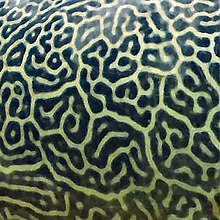
\includegraphics[width=0.6\textwidth]{220px-Giant_Pufferfish_skin_pattern_detail.jpg}
\end{minipage}
\begin{minipage}{0.5\textwidth}
\centering
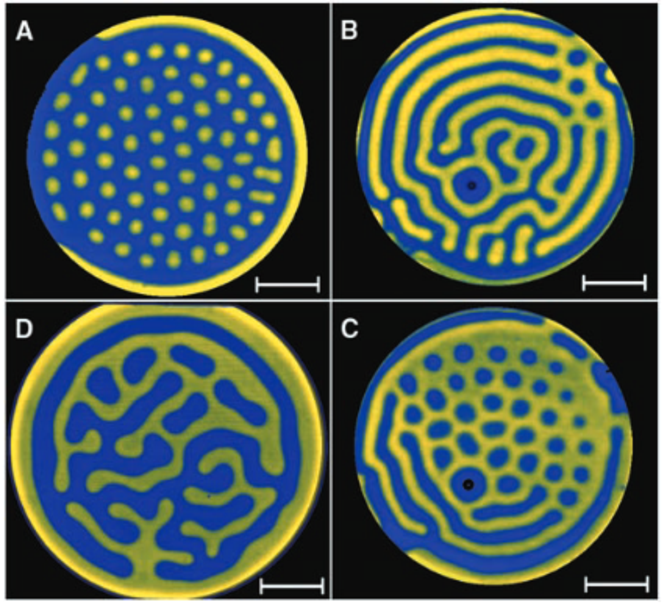
\includegraphics[width=0.7\textwidth]{turing_pattern_chem.pdf}
\end{minipage}
\caption{Motifs de turing sur la peau du poisson-globe, à gauche. A droite, motifs de turing émergeant d'une réaction chimique \cite{Horvth2009AnED}.}
\label{fig:turing_pattern}
\end{figure}

Qui dit système complexe dit système modulaire ?
Réseaux sociaux, communautés de fourmis, autant d'exemples montrant une emergence auto-organisée de modules. 


Système complexe adaptatif (cas) introduit par john Holland et Murray gellmann.
Ces systèmes sont un sous ensemble des systèmes complexes. Il s'agit de systèmes multi-agents qui réagissent à leur environnement, et s'auto-influencent. Ils se distinguent par l'émergence de propriétés et l'auto-organisation. C'est précisément ce qu'on cherche à faire dans un réseau de neurones. On dira qu'il y a eu un apprentissage si l'évolution du système a conduit à l'émergence de propriétés montrant une généralisation d'information sur les données présentées. 



Définir un système complexe : 

\subsection{Auto-organisation et emergence}

Développer ici ce qu'on appelle "auto-organisation", dans quel contexte c'est observé, des structures sociales aux dépliement de protéines. 
"Holisme": le tout est plus que la somme des parties

→ Auto-organisation definition

Les phénomènes d’auto-organisation sont déjà un élément caractéristique des systèmes complexes : Alan Turing montre qu’a partir d’un état presque uniforme de composants chimique, leur réaction et diffusion crée des motifs répétés. Ces motifs sont créés a partir de règles locales, on est bien sur un phénomène auto-organisé. Plus surprenant ces motifs appelés “turing patterns” sont présents dans de nombreux systèmes biologiques, par exemple sur la peau des animaux. Cela montre la prévalence des phénomènes d’auto-organisation dans la nature. 

A partir de règles locales, des comportements globaux peuvent donc émerger, de façon auto-organisée. Un des exemples biologiques montrant cette complexité est ainsil le cerveau humain. 

\subsection{Motivations pour les inspiration biologiques de l'intelligence artificielle}



\subsection{Questionnement du chapitre}

Ce chapitre questionne l'intéret de s'inspirer de la biologie : 
- pour développer une intelligence artificielle, et pourquoi on cherche a développer une intelligence artificielle, en fait ? 
- mais aussi les intérets plus généraux d'étudier les réseaux biologiques, pour une meilleure compréhension des systèmes auto-organisés par exemple. 

%%%%%%%%%%%%%%%%%%%%%%%%%%%%%%%%%%%%%%%%%%%%%%%%%%%%%%%%%%%%%%%%%%%%%%%%%%%%%
% SECTION 1 : définitions et propriétés
%- Tour d'horizons des définitions : en bio, en ingénieurie. Auto-organisation, conséquence de la modularité ? 
%- Taxonomie : fonctionnelle, stucture modulaire,emergence 
%- Position de l'autrice du manuscrit sur la modularité, intéret des différentes modularités
%- Discussion : est ce que notre esprit modulaire veut trouver de la modularité a tout prix ? ( quand la mod est fonctionnelle, peut etre biais de nos représentations ? Mais, on observe assez objectivement des modules physiques via les connexions dans de nombreux réseaux. Evolution l'a fait comme ca, probablement une réponse globale a un problème. 
%- Echelles de la modularité. 
%- Activation d'autres modules
%- Mutli-modalité - un mot, rappel dans une autre partie
%%%%%%%%%%%%%%%%%%%%%%%%%%%%%%%%%%%%%%%%%%%%%%%%%%%%%%%%%%%%%%%%%%%%%%%%%%%%%%%

\section{Quelle définition de la modularité ?}

L'étude de la modularité des systèmes est vaste. Entre étude des systèmes biologiques, ingénieurie des réseaux de neurones, ou même sociologie, les définitions de modularité varient. Nous chercherons donc dans cette partie à exhiber des définitions et des spécificités de ce qu'on appelle modularité.

\subsection{Modularité structurelle}

Lorsque le système possède une structure définie de réseau, typiquement un réseau de neurones, on peut définir une modularité en terme de graphe. Un système modulaire est ainsi \emph{Un système qui a une structure de graphe modulaire}.
Même en tant que graphe, modulaire est un terme large. De nombreux travaux proposent "une architecture modulaire" sans vraiement définir ce terme. 

\subsubsection{Mesurer la modularité structurelle d'un réseau}

La modularité d'un réseau est définie en théorie des graphes par le fait de pouvoir détecter des zones fortement connectées au sein de ce réseau, reliées par peu de connexions. Il s'agit donc de détecter des cliques, des sous-graphes fortement connectés, et de les différencier des zones moins connectées. 
La quantité la plus largement utilisée pour définir la	modularité d'un graphe est le \emph{coefficient de clustering}. Ce coefficient mesure la probabilité que deux noeuds soient directement connectés en sachant qu'ils ont un voisin en commun. Les réseaux sociaux par exemple, présentent des forts coefficients de clustering. D'autres mesures sont possibles, menant à une détection de zones fortement connectées. Cette modularité peut également se mesurer en regardant la densité des arêtes dans une partition du graphe, relativement à ce qu'on attendrait dans un graphe aléatoire. 

%\cite{Harriger2012RichCO}-> mesure modularité dans le cerveau, partie "méthodes" explique les méthodes de mesure de modularité. TODO les lister

\subsubsection{Réseaux en "petit-monde"}

La modularité d'un réseau est reliée à la propriété de petit-monde d'un graphe. 
Un graphe en \emph{petit-monde} (small-world network) est un graphe dans lequel la distance moyenne entre deux noeuds est proportionnelle à $\log(N)$, $N$ étant le nombre de noeuds du graphe. En d'autres termes, c'est un graphe dans lequel on trouvera forcément un chemin assez court relativement à la taille du réseau, entre n'importe quels noeuds. Un exemple typique de réseau en petit monde est celui des relations sociales avec la règle des "six degrés de séparation" mis en lumière par Stanley Milgram en 1967 \cite{Milgram1967TheSW} : en prenant deux individus au hasard aux états unis, Milgram montre qu'on peut les relier de connaissance mutuelle en connaissance mutuelle en, en moynenne, 6 étapes. Maintenant que la plupart de nos connaissances sont en enregistrées sur les réseaux sociaux, cette distance, entre tous les utilisateurs de facebook dans le monde entier, a été mesurée comme étant 3.5 degrés de séparation en 2016 \footnote{\url{https://research.fb.com/three-and-a-half-degrees-of-separation}}. La propriété de petit-monde est mesurée par le \emph{coefficient de petit-monde} $\sigma$. Il se mesure en comparant des métriques du graphe avec celles d'un graphe aléatoire équivalent, c'est à dire un graphe aléatoire ayant le même nombre de noeuds et la même densité de connexions. 
En notant $C$ le coefficient de clustering du graphe, $C_r$ celui d'un graphe aléatoire équivalent, $L$ la longueur (nombre d'arête) moyenne du plus court chemin entre tous les noeuds du graphe, et $L_r$ cette longueur dans un graphe aléatoire équivalent. 

$$\sigma = \frac{\frac{C}{C_r}}{\frac{L}{L_r}} $$

Un réseau est dit petit-monde si $\sigma > 1$, autrement dit, si la longeur du plus court chemin est inférieure à celle d'un graphe aléatoire, et/ou si le graphe présente plus de communautés qu'un graphe aléatoire. Cette métrique est cependant assez limitée, et il est plus judicieux existe d'autres mesures, comparant cette fois le coefficient de clustering et la longeur moyenne du plus court chemin à des graphes équivalents en treillis en plus des graphes aléatoires. 

Un réseau petit-monde n'est pas forcément modulaire. Par contre, un graphe ayant une structure modulaire, avec des communautés fortement connectées, est petit-monde. Un exemple est donné en figure~\ref{fig:graphe}. Le réseau $(b)$ est petit-monde : on trouve forcément un chemin court entre deux noeuds. Le réseau $(c)$ est également petit-monde, mais présente aussi des sous-graphes fortement connectés. 
La propriété de petit-monde semble avoir des avantages computationnel et se retrouve ainsi dans de nombreux exemples de réseaux biologiques. Nous détaillerons cet avantage en partie suivante. 

\begin{figure}
\centering
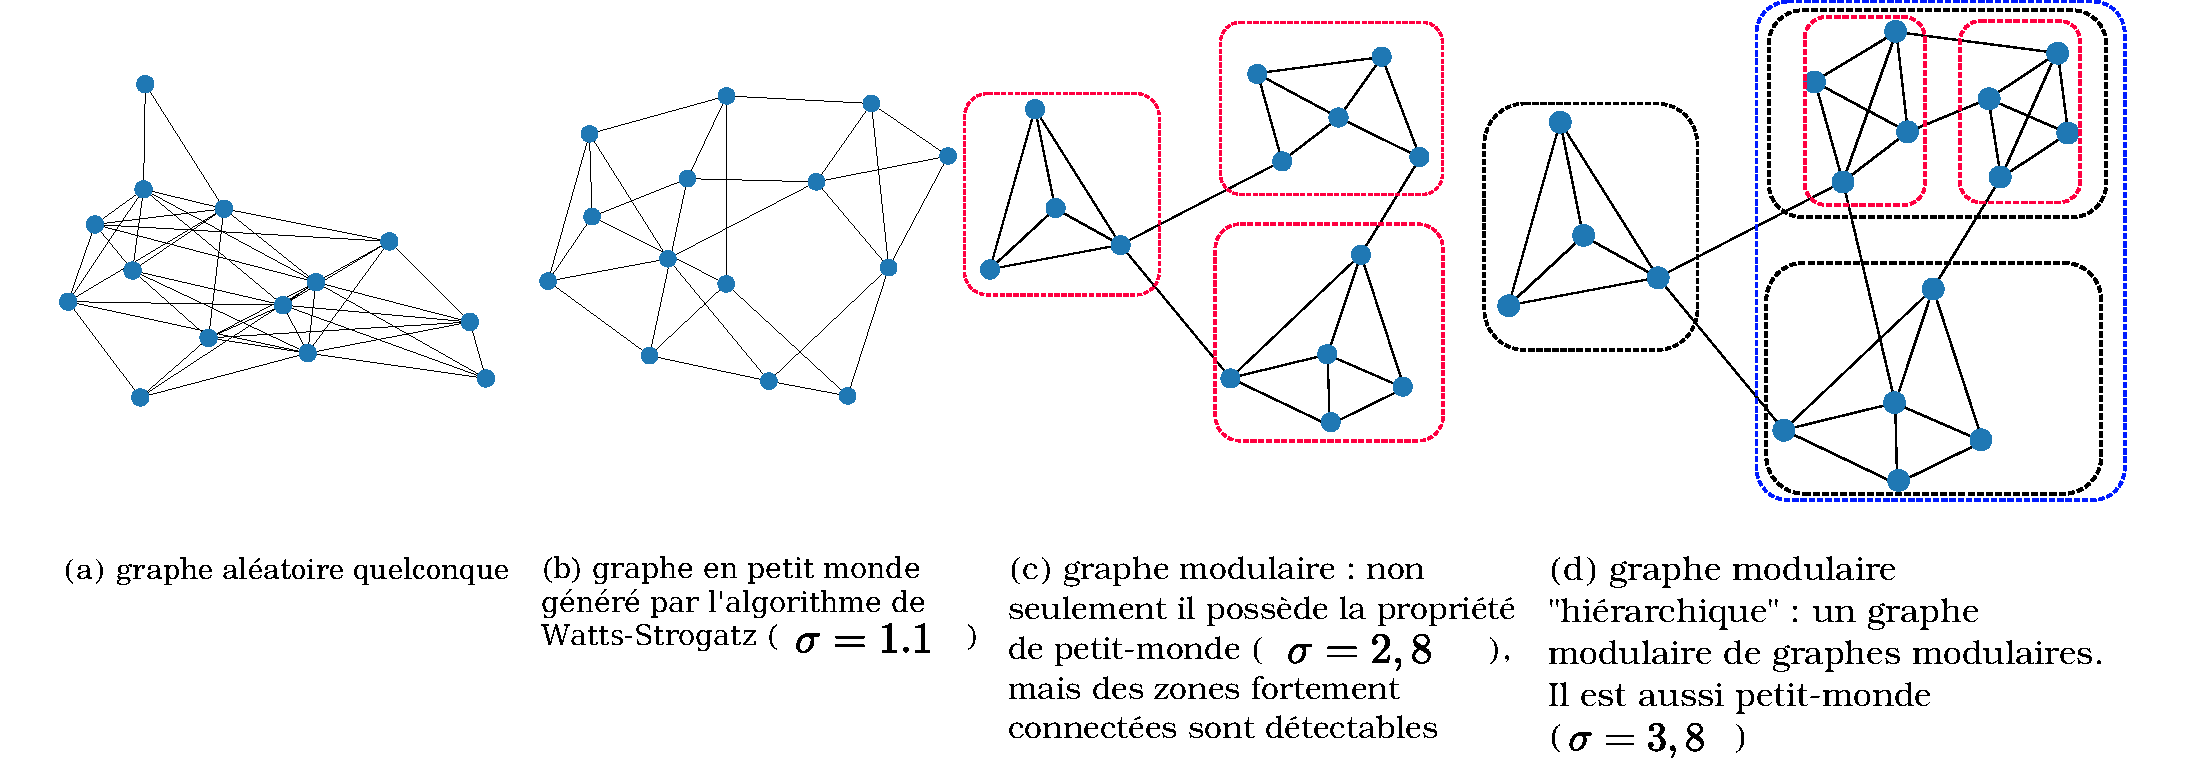
\includegraphics[width=\textwidth]{types_graphes.pdf}
\label{fig:graphe}
\caption{Exemples de graphes $(a)$ aléatoire, $(b)$ en petit monde, $(c)$ modulaire et $(d)$ modulaire hiérarchique.}
\end{figure}


\subsubsection{Modularité auto-similaire}

Si on prend un sous-graphe fortement connecté d'un graphe modulaire, ce sous-graphe peut éventuellement, à son tour, présenter une structure modulaire. On peut alors parler de modularité \emph{hiérarchique}, ou \emph{auto-similaire}. L'auto-similarité renvoie au processus de construction dans lequel on connecte par une arête deux structures jumelles (par exemple deux graphes complets); on copie ce graphe et on le connecte par une arête à sa copie pour former un graphe plus grand, etc. On gardera le terme auto-similaire pour parler de graphes formés de modules de modules, même si ces modules ne sont pas des copies exactes d'eux mêmes à différentes échelles, afin de garder le terme hiérarchique pour d'autre structures. Cette modularité "à différentes échelles" est souvent présente dans les réseaux. Le cerveau est par exemple souvent présenté comme un réseau modulaire auto-similaire \cite{Meunier2010ModularAH}. Des modules larges (aires fonctionnelles) sont formés de sous-modules, eux mêmes décomposables en sous-modules, etc. 

\subsubsection{Réseaux invariant par échelle}

Un dernier type de réseau à relier à la modularité sont les réseaux sans échelles (\emph{scale-free networks}). Un réseau small world est un réseau dont le nombre de noeuds de degré $k$ suit une loi de puissance. Les réseaux sans échelles ont notamment été étudiés par Barabasi lors de l'étude du world wide web, \cite{Barabasi2003ScaleFreeN}.
Ces réseaux sont "ultra-modulaires", ils ont un coefficient de clustering élevé. Il se caractérisent par la présence de sous-graphes ultra-connectés par des \emph{hub}, un noeud qui connecte d'autres noeuds moins connectés. Par leur distribution de connexions, on retrouve également dans ces réseaux une propriété d'auto-similarité: un sous-graphe autour d'un hub présentera une structure similaire à un sous-graphe plus grand, centré sur un plus gros hub, les hubs étant reliés entre eux. Par cette modularité, ils présentent donc aussi une caractéristique de petit-monde. Ces réseaux sont répandus au sein des structures sociales, par exemple les réseaux de citations entre articles scientifiques, les réseaux sociaux.

\subsubsection{Conclusion}

Un réseau dit "modulaire" exhibe donc souvent d'autres topologies plus spécifiques, telles que la propriété de petit-monde ou de réseau invariant d'échelle. Ces topologies sont détectées par différentes métriques s'appuyant sur les connexions sur réseau. Ces topologies se recoupent, un réseau modulaire étant généralement petit-monde, et un réseau invariant d'échelle ou modulaire hiérarchique étant modulaire. 
La modularité et ces topologies induisent des propriétés particulières dans les dynamiques de graphe, décrites en partie suivante. Les réseaux existant réellement, tels que les réseaux de neurones biologique, les réseaux sociaux, semblent partager ces structures très spécifiques que sont la modularité hiérarchique et l'invariance d'échelle \cite{Harriger2012RichCO, Meunier2010ModularAH, Clauset2008HierarchicalSA, Ravasz2002HierarchicalOO}. Ces structures sont donc génériques dans la nature. 

\subsection{Modularité fonctionnelle}

Nous avons vu que des réseaux peuvent être définis de modulaires dans la partie précédente ; cette décomposition, cependant, n'est pas forcément unique et directe. 
Définition des système complexe selon Le Moigne : le système dépend de la question que l'on cherche a étudier. Le système est complexe, mais sa décomposition et son analyse dépendra complètement de la question. Il n'y a donc pas un système intrinsèquement modulaire mais une approche adaptée au problème qui permet une décomposition. JL Le Moigne, La modélisation des systèmes complexes. 
Selon lui, le système est complexe d'un point de vue de l'observateur, car les comportements qui agissent au sein du système semblent imprévisibles; par contre, on peut le décomposer pour le comprendre. 
Donc si on veut étudier un système "réel", sa modularité dépend en fait de ce qu'on veut étudier. 
Edgar Morin pensée complexe (?)

Différence structure/organisation -> A mettre dans modularité ?? 


Conclusion de la sous-section : la modularité d'un système complexe n'est pas forcément unique. Elle dépend de ce qu'on cherche à simuler ou étudier. Dans notre cas, on construira un système a partir de modules, on a donc une modularité directement définissable. Il semble cependant nécessaire de savoir la question que l'on cherche a étudier en définissant cette modularité. 

%\subsection{Modularité temporelle}
%
%Du point de vue du système dynamique, l'aspect temporel n'est finalement qu'une dimension de plus dans la modularité du système. Les règles locales faisant évoluer le système dynamique amènent à des comportements complexes temporellement parlant. Par exemple, un attracteur fractal est le résultat des trajectoires d'un système dynamique complexe à l'état de chaos. 
%
%La modularité s'associe aux séquences dans le cerveau. Les mémoires, l'interaction entre échelles de fonctionnement apportent une modularité supplémentaire.

\subsection{Emergence d'une modularité et auto-organisation}

L'aspect complexe et modulaire d'un système peut aussi être étudié via les propriété qui en émergent, notamment l'auto-organisation.

Système complexe = interaction entre de nombreux élements. Mais on pourrait totalement imaginer que ces interactions mènent à une sorte de désordre. Or, des motifs apparaissent, partagés par de nombreux systèmes. C'est ce qu'on appelle auto-organisation. 




% SECTION 2 introduction via la biologie, exemples 
%%%%%%%%%%%%%%%%%%%%%%%%%%%%%%%%%%%%%%%%%%%%%%%%%%%%%%%%%%%%%%%%%%%%%%%%%%%%




\section{La modularité, répandue dans les système biologiques}

% Passer cette partie après la section définition ???
\subsection{Le cerveau, réseau modulaire fondamental}

Un neurone est un système dynamique, donc l’activité electrique est régie par des équation d’évolution dépendant des connexions qu’il recoit. Le cerveau dans son ensemble est alors,  fondamentalement, un agrégat de neurones. 300 neurones dans le ver microscopique  Caenorhabditis elegans, un million dans le cerveau des insectes, jusqu’a 86 millards de neurones dans un cerveau humain. Tous ces pics electriques et chimiques nous permettent une prise de décision, une mémoire, de la réflexion, des représentations …. Un ensemble de capacités que l’on nomme intelligence. Cette intelligence n’est pas localisée à un endroit précis dans le cerveau, de ce qu’on sait. Elle résulte de l’activité globale de l’ensemble de neurones, et est ainsi une propriété émergente. 

Cet amas est le point de départ des études autour de l’intelligence artificielle. Si on veut créer un systèmes ayant une intelligence émergente, il nous faut comprendre les mécanismes de cette émergence, et donc comprendre les systèmes existant ayant cette capacité. Les réseaux de neurones se sont donc d’abord inspirés du cerveau avant d’être développés plutot sur un aspect computationnel avec moins de vraisemblance biologique.
Cette inspiration biologique ne se limite pas à assembler des neurones : l’architecture cérébrale à plus grande échelle est aussi une source d’inspiration dans la recherche de systèmes intelligents, autrement dite, intelligence artificielle.  
Et le cerveau semble avoir une architecture particulière : il est modulaire, à plusieurs échelles. 
Les premières propositions de modèle du cerveau humain datent du début du XXeme siècle. Déjà, un découpage en aires est proposé pour expliquer le fonctionnement de cet organe, notamment avec les travaux de Broca et Wernicke qui mettent en lumière des zones du cerveau qui semblent responsable du langage. Le modèle connexioniste du cerveau, formalisé à partir de ces travaux par Geschwind dans les années 60 , décompose ainsi le langage en plusieurs fonctions : la compréhension, la lecture et l'action de parler. Ce modèle n'est plus vraiment utilisé, mais l'idée de décomposition en modules reste valable.
Avec l'avènement des outils d'imagerie, le cerveau a pu être cartographié plus préciséement en un ensemble d'aires, agissant comme modules fonctionnels au sein d'une structure complexe; ces aires sont elles mêmes composées de modules distincts. 

L'étude des aires et des connexions entre zones du cerveau, comme~\cite{primate_cortex_91} dans le cas du cortex visuel du primate, découpent les zones activée pour la vision en modules distincts, et montrent que ces modules sont connectés. Ces connexions, en fonction des modules, sont réciproques ou non. Les "pathsways" du cerveau désignent des modules fortement connectés. Leur détection expérimentale est réalisée en relevant des indicateurs de dépendance (corrélation, ..., en fonction des méthodes utilisées). Ainsi, \cite{Rolls2002ComputationalNO} précise la structure des différentes aires cérébrales en présentant les connexions au sein de ces aires, par exemple la structure présentée en figure~\ref{fig:cortex2} pour l'aire visuelle. 
Les connexions du cerveau sont présentes à différentes échelles: des pathsways existent ainsi au sein de l'aire visuelle du cerveau, mais des boucles de rétroaction entre zones cérébrales sont présentes à plus grande échelle, par exemple la boucle baso-thalamo-corticale. Ces différentes échelles au sein du cerveau amènent \cite{Meunier2010ModularAH} à le présenter comme un réseau "hiérarchique modulaire". Cette activité "sans échelle" pourrait notemment permettre au cerveau d'appréhender les notions temporelles, transposant ainsi un réseau spatial en une activité temporelle \cite{biyu_scale-free_2014}.

La structure cérébrale est donc bien particulière. Aussi, l'inspiration cérébrale des modèles d'intelligence articielle ne se résume pas au modèle neuronal, les éléments architecturaux et de connexions sont donc à considérer. 
\begin{figure}[t]
\centering
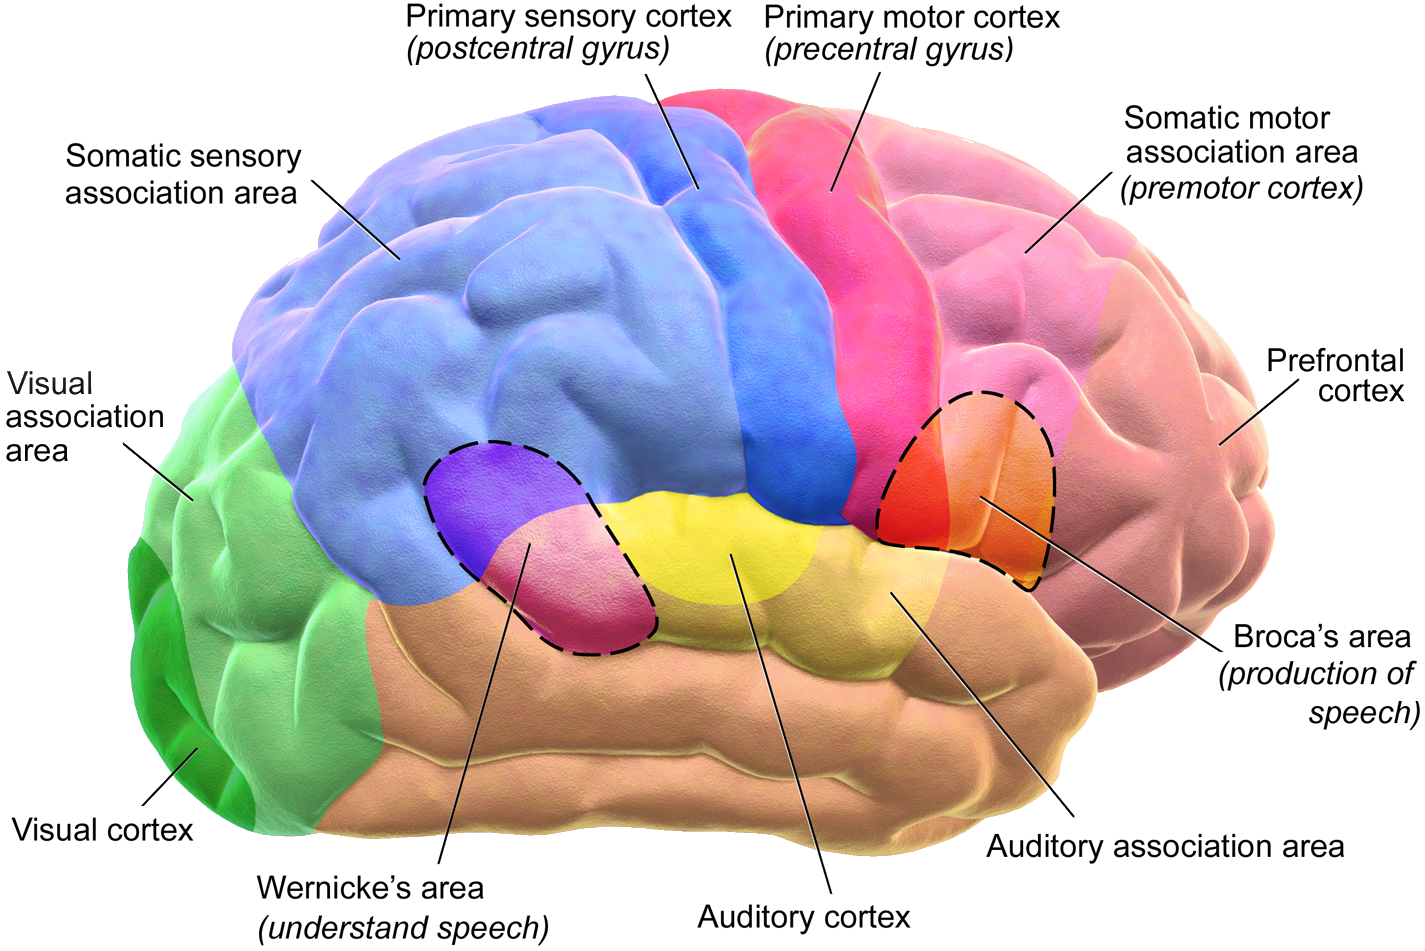
\includegraphics[width=0.5\textwidth]{Blausen_0102.png}
\caption{Aires du cerveau humain}
\end{figure}

\begin{figure}[t]
\begin{minipage}{0.5\textwidth}
\centering
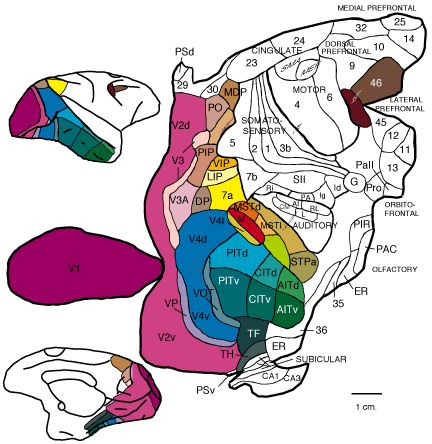
\includegraphics[width=0.7\textwidth]{FVE_fig2map.png}
\label{fig:cortex1}
\end{minipage}
\begin{minipage}{0.5\textwidth}
\centering
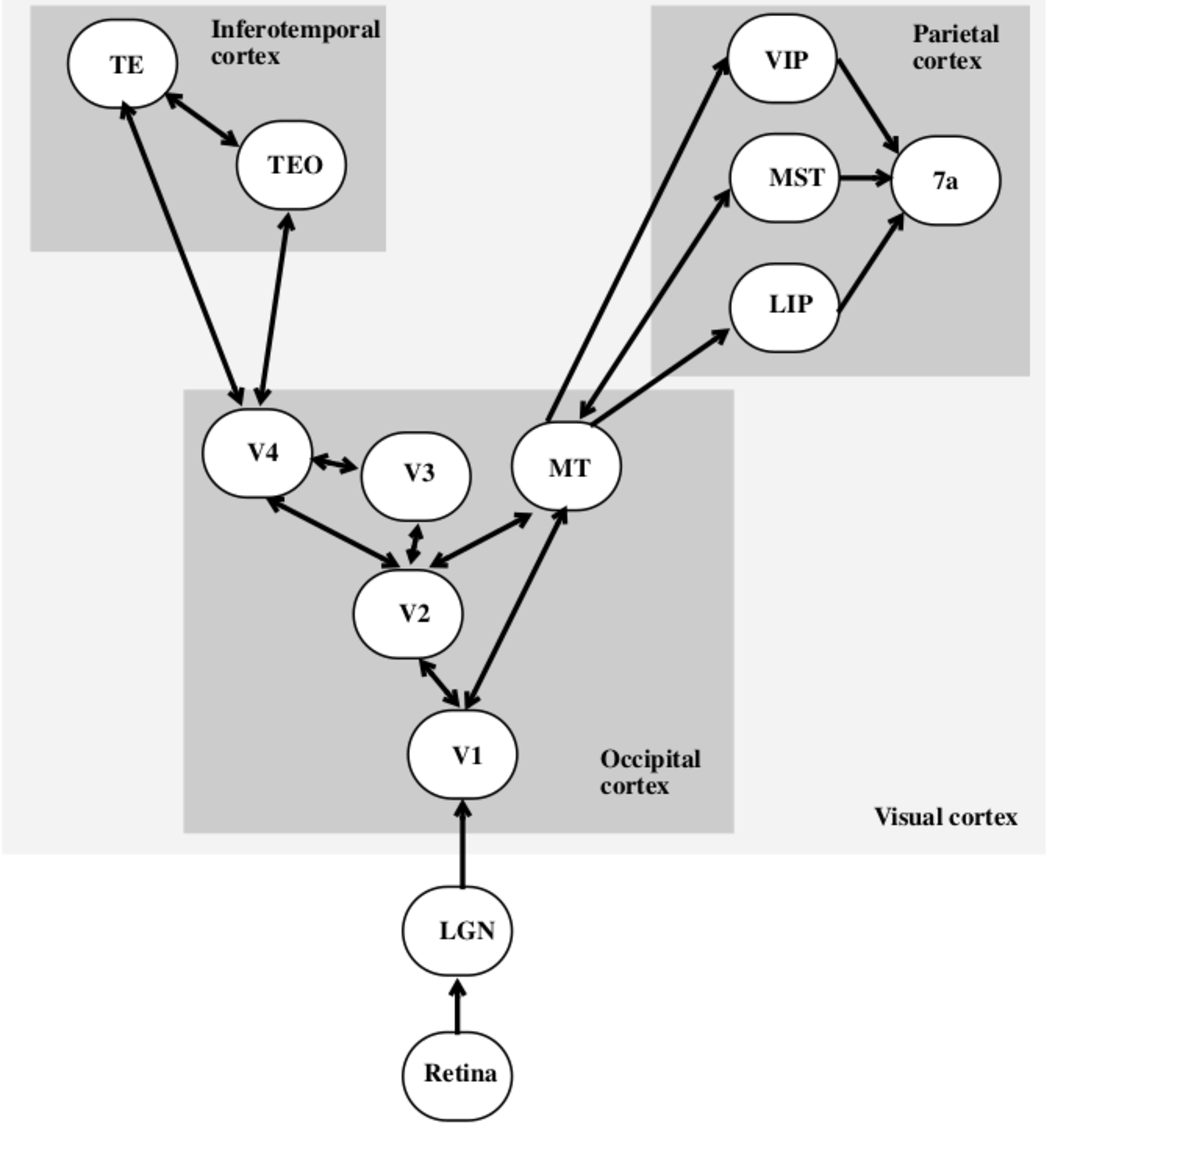
\includegraphics[width=0.8\textwidth]{rolls_pathways.pdf}
\label{fig:cortex2}
\end{minipage}
\caption{carte aplanie des aires du cortex visuel du macaque \cite{primate_cortex_91}, à gauche, et pathways dans ce cortex visuel entre les aires à droite \cite{Rolls2002ComputationalNO}. L'architecture neuronale présente des rétroaction entre zones, dans une architecture non-hiérarchique.}
\end{figure}

 
%- Nombreuses études s'appuient sur le système modulaire : le cerveau \cite{primate_cortex_91,mountcastle_columnar_1997,binzegger05}
%
%
%- Modularité hiérarchique( modules de modules) -> Ajouter infos depuis l'article qui parle de modules hiérarchiques. 
%%Ajouter figure du cerveau avec le schéma des aires
%
%Finalement : 
%Cerveau présente ce qu'on peut appeler des modules, avec des connexions entre eux, avec rétroaction. 
%
%Leur mesure peut etre structurelle (regarder les structures de neurones), ou fonctionnelle : quelles aires s'activent pour une fonction ? \\
%Détail des types de modularité en parties suivantes. 

\subsection{Des réseaux et des modules dans tous les systèmes biologiques}

Les phénomènes émergents ne se limitent pas au cerveau : tous les systèmes biologiques semblent présenter des fonctionnement issus de systèmes complexes, menant à une régulation globale d'une quantité, à un comportement commun, autrement dit, l'émergence d'un comportement. On peut par exemple citer l'exemple des nuées d'oiseaux : des centaines ou des milliers d'oiseaux peuvent voler ensemble, sans se heurter ni se disperser, le tout sans avoir d'instructions globale. Cette capacité à rester en nuée émergent des règles locales que connaissent chacun des oiseaux. Ces règles régissent le comportement individuel à avoir avec leur voisins proches. Ces règles simples permettent à ces milliers d'individus de voler en groupe et de se déplacer.
Les arbres en forêt s'adaptent, pour pousser sans se toucher, et partageraient même des information en communiquant. Sans forcément parler d'intelligence, on peut tout à fait voir en ces comportement des mécanismes émergents.


%%%%%%%%%%%%%%%%%%%%%%%%%%%%%%%%%%%%%%%%%%%%%%%%%%%%%%%%%%%%%%%%%%%%%%%%%%%%%%%%%%%%%%%%%%%%%%%%%%%%%%%%%%%%%%%%%%%%%%%%%%%%%%%%%%%%%%%%
% SECTION 3: quel intéret à utiliser des architectures modulaires pour l'apprentissage ? 
% - 
%%%%%%%%%%%%%%%%%%%%%%%%%%%%%%%%%%%%%%%%%%%%%%%%%%%%%%%%%%%%%%%%%%%%%%%%%%%%%%%%%%%%%%%%%%%%%%%%%%%%%%%%%%%%%%%%%%%

\section{Intérêt computationnel des réseaux modulaires, et comment les construire}

Les réseaux modulaires sont ainsi prépondérants dans les systèmes "réels", les systèmes présents dans la nature (réseaux de neurones, biologiques...) ou les réseaux émergents de l'interaction entre humains (réseaux sociaux, réseaux des citations entre auteurs). On retrouve dans tous ces réseaux une structure commune modulaire hiéarchique, parfois avec un aspect invariant d'échelle, les réseaux présentant des hubs. Cette structure de réseau est loin d'un réseau aléatoire et a donc été sélectionné par l'évolution ou les interactions locales. On peut se demander si les réseaux biologiques résultant d'une évolution sélective sont modulaire parce que cette structure présente des avantages computationnels, ou si c'est parce qu'ils résultent d'une évolution sélective modifiant des parties du réseau, qu'ils sont modulaires. 
Ces avantages motivent l'idée de s'inspirer de réseaux réels pour créer des systèmes computationnels performants et émergents, notamment dans le cadre de l'intelligence artificielle. 

Barabasi : Hypothèse que les réseaux small world présentent un avantage evolutionnaire.
Modularité hiérarchique présente l'avantage de maintenir une activité dans le réseau sans que ca ne colonise tout ni ne s'eteigne, ce qui est nécessaire pour la computation. 



\subsection{réponse a un problème de contraintes physiques, énergétiques}


- Parallelisme, calcul et small world networks : réponse a un problème de contrainte physiques, énergétiques. 
- Calcul distribué 
- Automates cellulaires ?

- Exemple des puces neuromorphiques, calcul embarqué


Conclusion: En décentralisant le calcul, on cherche aussi à plus facilement l'utiliser via des architectures neuromorphiques. 

\subsection{Modularité, complexité et émergence d'un apprentissage }


Systèmes complexes et emergence: possibilité d'apprentissage, exemple du reservoir computing

La modularité est liée a la complexité des systèmes, donc l'emergence de comportements chaotiques et/ou synchronisés. 

SYSTEMATIC GENERALIZATION : WHAT IS REQUIRED
AND CAN IT BE LEARNED ? : 
Our findings show that the generalization of modular models is much more systematic and that it is highly sensitive to the module layout, i.e. to how exactly the modules are connected.

Simplicité de la modularité : exemple de construction des fractales, exemple du rigaudon

Parler des architectures de Hebb (précurseur) ici ou avant ?

slow intermodular processes, fast intramodular : la modularité spatiale a l'origine de différentes échelles temporelles \cite{Pan2009ModularityPS}


\subsection{Types de connexions}

Opaque vs tout savoir


\subsection{Modularité comme propriété émergente ou modularité définie}

On a défini un réseau modulaire en analysant sa structure ou sa fonction une fois créé. Néanmoins, la façon dont ce réseau a été élaboré peut résulter de plusieurs processus : l'aspect modulaire peut émerger d'une sélection, d'une construction ou d'un recablage des arêtes et des noeuds du graphe; ou alors la modularité peut être définie a priori par la structure du réseau. Cette distinction est nécessaire lorsqu'on cherche à créer des réseaux de neurones pour l'apprentissage, qui sont alors des systèmes qui s'adaptent. La structure peut donc être présente a priori et l'apprentissage uniquement créé par l'adaption de poids au sein du réseau, ou l'apprentissage passe également par l'adaptation des arêtes.
Au sein même des réseaux dont la structure est définie a priori, la \emph{fonction} de chaque module peut être définie ou non. Dans l'exemple le plus "prédéfini", le réseau d'interaction est défini en liant des modules ayant des fonctions bien précises. C'est le cas par exemple de l'organisation structurelle d'une entreprise, chaque agent ayant un role défini au sein d'une hiérarchie. Ce sont ce genre de modules prédéfinis qui ont été utilisés lors des débuts de la recherche en intelligence artificielle, dans les systèmes experts. Même si ces systèmes ne font pas d'\emph{apprentissage}, un comportement global émerge de l'interaction entre modules. Par exemple, Brooks \cite{brooks_sumsumption_85} propose une architecture en robotique appelée sumsumption, dans laquelle les comportements "intelligents" et haut niveau d'un robot ( "explorer", "planifier") émergent de la combinaison d'actions et de capteurs "bas niveau" comme "tourne", "avance", "faire demi-tour", "detection" (figure~\ref{fig:brooks}).

\begin{figure}
\centering
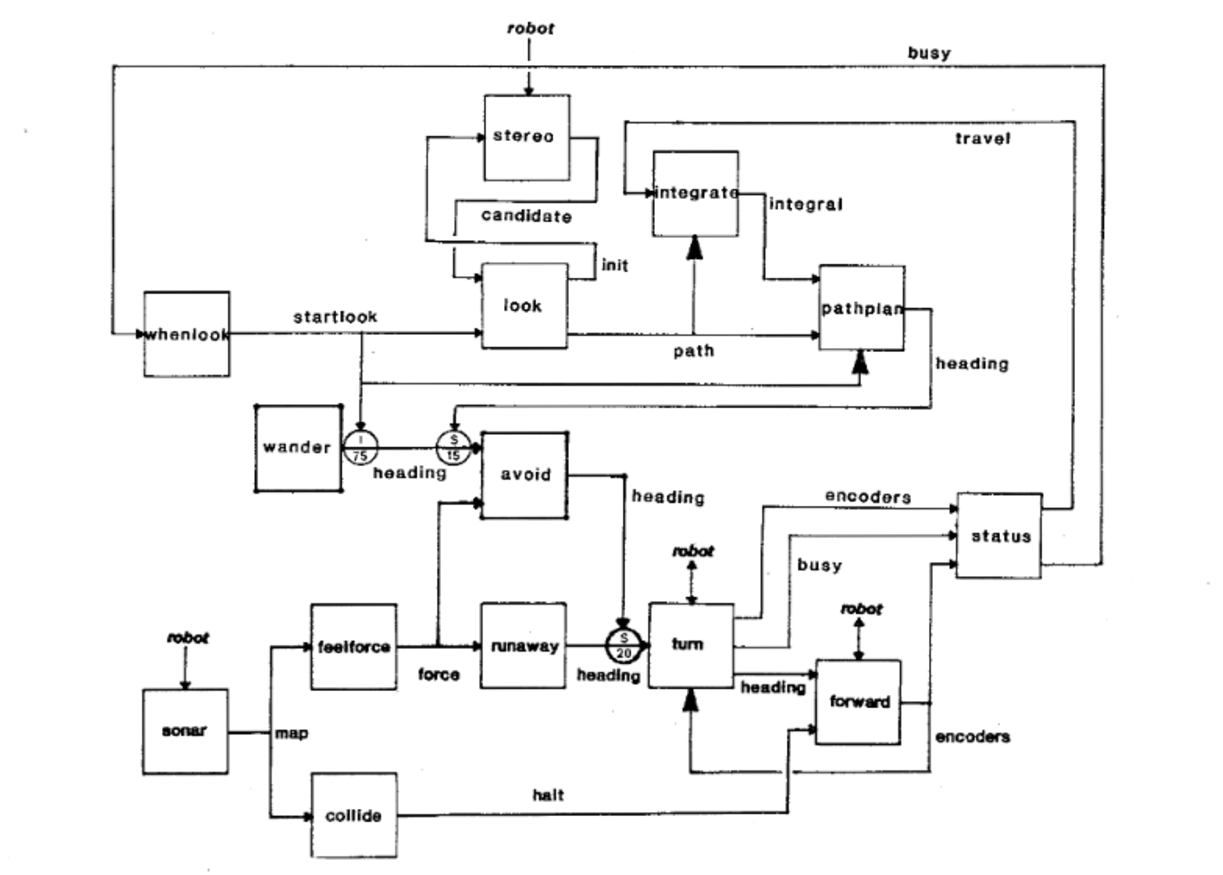
\includegraphics[width=0.5\textwidth]{brooks.pdf}
\caption{Architecture experte de Brooks. Les modules sont prédéfinis et codent chacun un comportement définis à l'avance. Ils sont connectés en un réseau cablé à l'avance. Cette ingénieurie permet à un robot d'avoir un comportement plus haut niveau que les modules bas niveaux encodés.}
\label{fig:brooks}
\end{figure}

Ces réseaux experts précablés ne font pas d'apprentissage. Une main ingénieure doit trouver les bons paramètres, les bonnes connexions, et les bonnes fonctions faisant émerger les comportement voulus. A l'ère de l'apprentissage, on peut remplacer ces modules dont la fonction est prédéfinie par des modules qui apprennent leur fonction. Ils sont alors connectés selon un réseau fixe, mais apprendront au sein de ce réseau leur fonction. 

Enfin, certains réseaux de neurones, bio-inspirés, renforcent une connexion lorsque deux neurones s'activent en même temps. C'est la règle de Hebb "neurones that fire together, wire together". Depuis un bouillon de neurones initial, l'état final du système présente une structure de réseau apprise.  -> Citer des exemples de réseaux qui adaptent des connexions. 


Attention : même avec une modularité prédéfinie, on reste un système complexe, donc on pourra avoir des propriétés d'adaptation émergentes.
 
%%%%%%%%%%%%%%%%%%%%%%%%%%%%%%%%%%%%%%%%%%%%%%%%%%%%%%%%%%%%%%%%%%%%%%%%%%%
% SECTION 4 En pratique, ou en est on des réseaux de neurones modulaires ?
%%%%%%%%%%%%%%%%%%%%%%%%%%%%%%%%%%%%%%%%%%%%%%%%%%%%%%%%%%%%%%%%%%%%%%%%%%%%%ùù

\section{Modularité dans les réseaux de neurones}

Au sein des systèmes complexes, les réseaux de neurones artificiels se sont directement développés en s'inspirant des réseaux biologiques. Hebb formule ainsi en 1949 "neurons that fire together, wire together". Les réseaux de neurones développés depuis sont alors inspirés de la biologie, en s'en éloignant plus ou moins. Quel que soit leur éloignement, ce sont des systèmes complexes dans le sens ou il s'agit d'un grand nombre de neurones reliés entre eux, et qu'on développe dans le but de l'émergence d'une propriété d'apprentissage et de généralisation.

Ces réseaux sont par exemple le perceptron, les cartes auto-organisatrices. 
L'intérêt de chercher des aspect modulaires des réseaux de neurones a été formulé par exemple par \cite{towards_novel_2001} : 

A partir du perceptron, les réseaux de neurones profond ont été développés comme une assemblée de perceptrons reliés hiérachiquement (fin 90 ) 

\subsection{Deep Learning}
Boites noires qui ont des performances remarquables sur tous les domaines, leur représentation et compréhension est quant à elle toujours un challenge. Ajouter un aspect modulaire non-hiérarchique dans les calculs de ce genre de réseau, pour augmenter la vitesse d'apprentissage ou encore pour 

\subsubsection{Réseaux de neurones profond et modulaires}

- Réseaux qui apprennent a s'organiser en modules. Interet. Limites ? Performances ? \cite{Andreas2016NeuralMN,Kirsch2018ModularNL}
"The NMN approach is intuitively appealing but its
widespread adoption has been hindered by the large amount of domain knowledge that is required
to decide (Andreas et al., 2016) or predict (Johnson et al., 2017; Hu et al., 2017) how the modules
should be created (parametrization) and how they should be connected (layout) based on a natural
language utterance. Besides, their performance has often been matched by more traditional neural
models" ( systematic generalization article ) 

\subsubsection{Utiliser des modules pour mieux représenter les réseaux de neurones profond}


- Trouver des modules dans les réseaux pour les expliquer ? \cite{Watanabe2018ModularRO,Csordas2021AreNN}
are neural net modular : "it uses different modules for very different functions = Pspecialize," et "it uses the same module for identical functions that
may have to be performed multiple times = Preuse"
- Reconciling deep learning with symbolic artificial intelligence: representing objects and relations(2019)
Pb du deep learning = Data inefficiency (comparé a l'humain);Poor generalisation; Lack of interpretability.

\subsection{Réseaux auto-organisés}

Les réseaux auto-organisés sont directement inspirés des réseaux biologiques. Au sein de ces réseaux
Plus qu'en deep learning, les réseaux de neurones auto-organisés
- Auto-organisation prend une profonde inspiration biologique, tout comme les modules.
- Exemple de réseaux auto-organisés modulaires : développer dans la partie suivante.
\begin{figure}
\begin{minipage}{0.5\textwidth}

%\centering
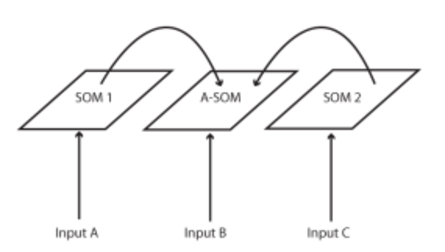
\includegraphics[width=\textwidth]{asom}
\caption{A-SOM model \cite{johnsson_associative_2009}}
\end{minipage}
\begin{minipage}{0.5\textwidth}
%\centering
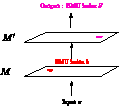
\includegraphics[width=0.9\textwidth]{hsom}
\caption{HSOM model \cite{LampinenClusteringPO}}

\end{minipage}
\end{figure}
\cite{LampinenClusteringPO}

\cite{parisiLL}

Lefort

Travaux préliminaires de l'équipe ->  Bassem, Ménard ?



\subsection{Construire une architecture modulaire}

A mettre dedans : 

- Réseaux top down / modulaires ? définition, a quel point un réseau est modulaire, qu'est ce qu'on appelle réseau modulaire ? 
Fonction définies au préalable vs émergence des fonctions. 
Modules définis au préalable vs émergence des modules. 


%%%%%%%%%%%%%%%%%%%%%%%%%%%%%%%%%%%%%%%%%%%%%%%%%%%%%%%%%%%%%%%%%%%%%%%%%%%%%%%%
% SECTION 5 : proposer des enjeux par rapports au réseaux listés précedemment 
%%%%%%%%%%%%%%%%%%%%%%%%%%%%%%%%%%%%%%%%%%%%%%%%%%%%%%%%%%%%%%%%%%%%%%%%%%%%%%%%


\section{Enjeux d'une architecture modulaire de SOMs}

On connait plutot bien les SOM, mais on sait que des comportements nouveaux peuvent émerger lorsqu'on met en interaction des systèmes étudiés séparément. 
On peut donc se poser la question des comportements qui peuvent survenir dans ce cas.

Dans les structures de cartes étudiés, modularité forte dans le sens ou les fonctions des modules sont prédéfinies. Si on ne fournit que les règles d"interaction, ou est ce qu'on se situe ? 
 
 
Position du manuscrit : architecture 
%%%%%%%%%%%%%%%%%%%%%%%%%%%%%%%%%%%%%%%%

Plan de la partie ! 

 

\begin{enumerate}
\item Intro : Notre monde est modulaire, en tout cas nous l'interprétons en tant que tel. Proposé déjà dans les années 60 - breve histoire des réseaux de neurones ?
Remarquer que nous, observeur, raisonne et se construit modualairement. Il nous est difficile de concevoir les choses autrement. 
Les disciplines sientifiques par ex, un domaine obéit a des principes
\item Qu'appelle t-on la modularité ? Définitions claires et propriétés
	\begin{itemize}

		\item Definition
			\begin{enumerate}
			\item Structurelle, dans les systèmes réseaux
			\item Fonctionnelle, dans les systèmes dont on ne connait pas la structure ?\\
			\item Temporelle / mais est ce que le temps ce n'est qu'une dim de plus
			\item Modularité hiérarchique attention : deux defs a hiérarchiques. Soit c'est une histoire de connexions, soit d'auto-similarité. On parle nous de l'auto similarité !!! Au contraire l'autre forme de hiérarchie n'est pas observée en bio.
			\end{enumerate}
		
		\item Propriétés de la modularité 
			\begin{enumerate}
			\item Auto-organisation
			\item Types de connexions
			\item Emergence
			\end{enumerate}
	\end{itemize}	
\item Exemples Biologiques et computationnels
	\begin{enumerate}
	\item Biologie : opti evolution a priori...
	\item Computationnel : pareil.
	\end{enumerate}
	
\item Maintenant qu'on sait ce que sont les systèmes modulaires, en quoi on peut faire de l'apprentissage avec ? Quels sont les intérêts ?
	\begin{enumerate}
		\item Exemples de réseaux auto-organisés
		\item Exemples de réseaux de neurones : deep learning
	\end{enumerate}

\end{enumerate}






\chapter{Cartes de Kohonen et modèle d'architecture CxSOM}
\graphicspath{{02-SOM/}}
\minitoc
\comment{Idée du chapitre : 

"Qu'est ce qu'on veut faire avec des cartes de Kohonen ?" 
" A quoi servent les cartes de Kohonen ?" ok on les utilise pour de la visualisation, de la réduction de dimension. La visualisation est bien pour un observateur humain, la réduction de dimension peut impliquer qu'on va utiliser un algorithme derrière. Mais les cartes de Kohonen vont plus loin dans l'apprentissage: on a une approximation de l'espace d'entrée par un graphe. Cela veut dire qu'une entrée est associée à un prototype dans la carte, mais inversement : un prototype est associé à un ensemble d'entrée continu ou contigu.
Une entrée est alors représentée par notamment sa position dans la carte : un nombre donc, ou une paire. 
Il est possible de faire du calcul sur ces positions au sein d'algoithmes. 
Dans cette thèse, on a pensé à utiliser cette propriété pour construire un réseau de cartes auto-organisatrices. Par ce réseau, on peut exploiter les positions pour générer des dynamiques au sein de la carte qui permettront une prise de décision, ou des représentation de donnée différentes. 
// Kohonen : il faut surprendre encore ! Par quel 
bout le prendre ? 
→ Appuyer sur les cartes 1D
→ Comment ca se fait qu’on les utilise pas de ouf ? 
→  Intérêt de la topologie de la carte. Dans une carte seule, est ce que c’est vraiment utile ?
→ Questionnement informatique : qu’est ce qui se passe en fait dedans, mais c’est quand même rigolo. }


\section{Carte de Kohonen}

\subsection{Algorithme et notations}

Rappelons les notations concernant une carte de Kohonen standard. Prenons un ensemble de données d'entrées, dans lequel chaque élément est un vecteur d'un espace $D$, dans lequel est définie une distance $d$.
La carte de Kohonon construite sur ces entrées est un graphe, généralement une ligne 1D ou une grille 2D de $N$ noeuds. Chaque noeud possède un poids associé $\w_e in D$ ou \emph{prototype}, du même espace que les entrées. et une \emph{position} $i$ dans la carte. Ces positions sont ensuite indexées entre $0$ et $1$ par $p= \frac{i}{N}$ pour l'homogénéité des calculs. 
L'ensemble des poids est noté ${\w_e(p), p \in [0,1]}$. 
L'algorithme se décompose de la façon suivante :

\begin{enumerate}
\item Une entrée $\inpx_t$ est présentée à la carte.
\item L'unité ayant le poids le plus proche de $\inpx_t$ selon la distance $d$ est choisie comme \emph{Best Matching Unit} de la carte. Sa position est notée $\bmu$.
\item Chaque poids $\w_e$ est déplacé vers l'entrées $\inpx$, en fonction de sa distance dans la carte à la best matching unit : 
\begin{equation}
\w_e(p,t+1) = \w_e(p,t) + \alpha h(\bmu,p)(\inpx - \w_e(p,t))
\label{eq:update}
\end{equation}
\end{enumerate}

$h(\bmu,p)$ est la \emph{fonction de voisinage}. Elle est maximale en $p = \bmu$ et décroissante autour de cette position. Dans notre étude, les fonctions de voisinage sont triangulaires, donc maximales en $\bmu$, décroissante sur le rayon de voisinage $h_e$ et nulle après.

Lors de l'étape 2 de l'algorithme, une activité peut être calculée, au lieu d'une distance pour choisir le BMU. Ce dernier est alors choisi comme $\bmu = \argmax_p (a(\inpx,p)$. Nous utiliserons cette solution dans notre modèle. Les notations au sein d'une carte sont résumées en figure~\ref{fig:one_map_not}.

\begin{figure}
\centering
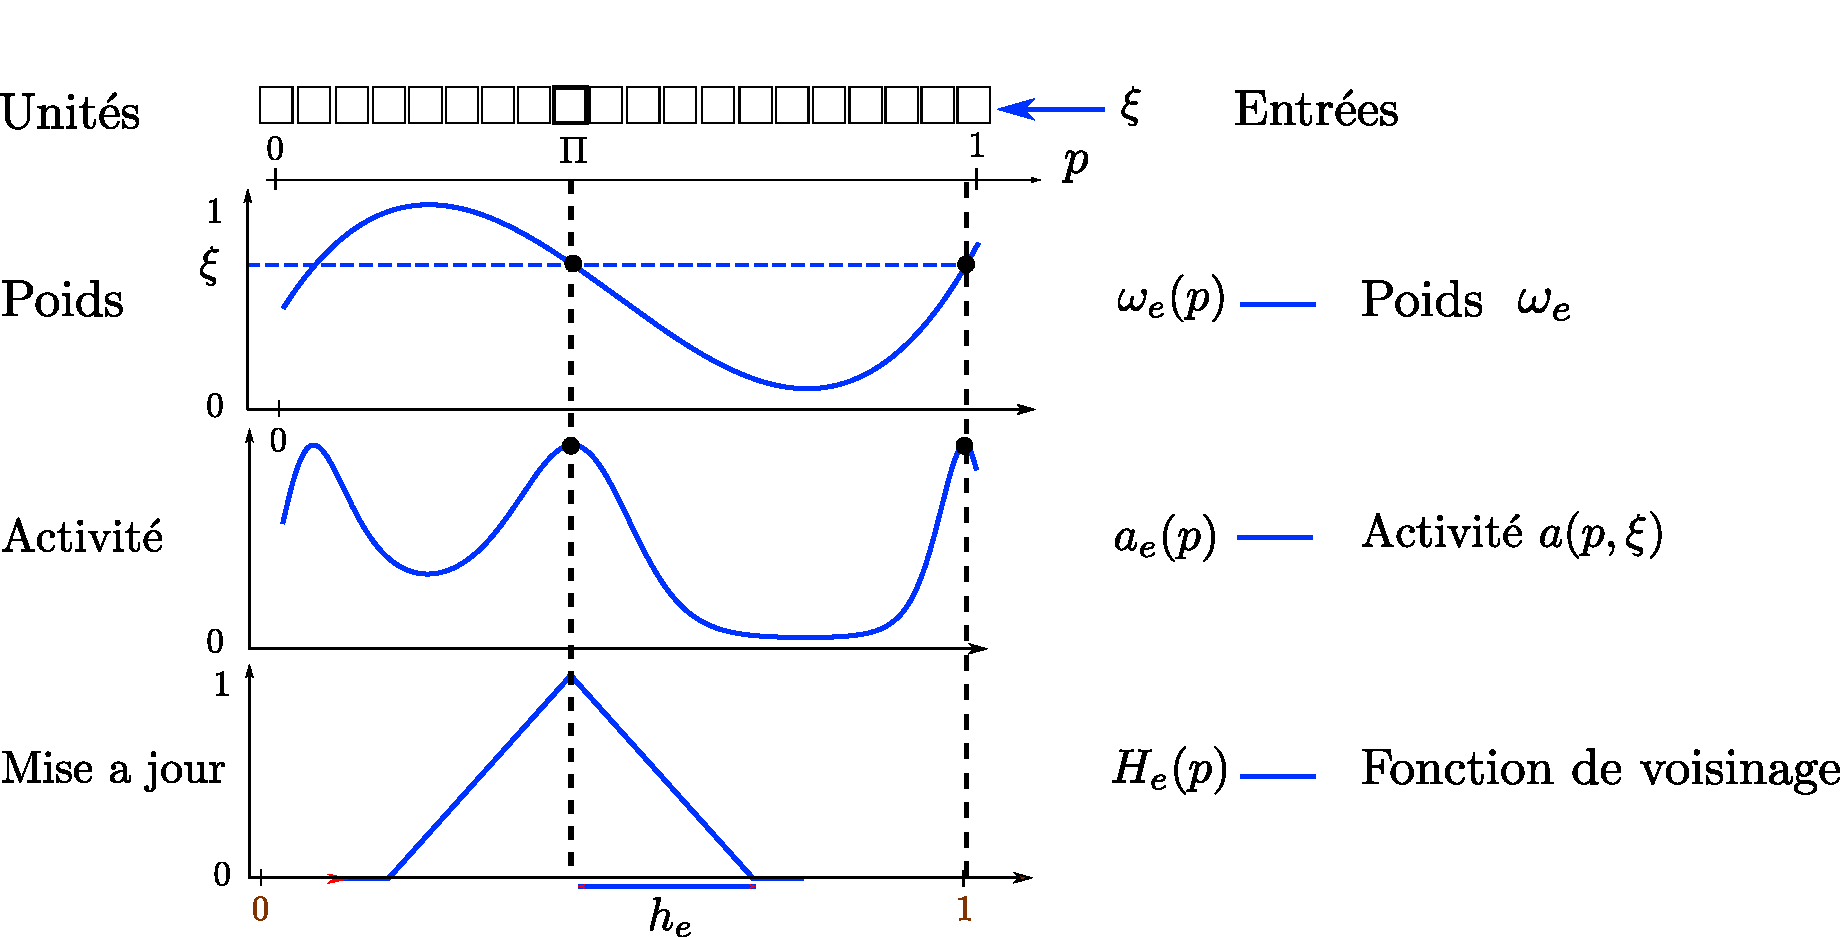
\includegraphics[width=0.6\textwidth]{one_map_one_layer.pdf}
\caption{Notations utilisées dans une carte de Kohonen simple}
\label{fig:one_map_not}
\end{figure}


\subsection{Approche topologique des cartes de Kohonen}

\draft{La notion de voisinage et de topologie est un élément clé des cartes de Kohonen. Le voisinage est en effet pris en compte lors de l'apprentissage et lors de l'interpretation des cartes. Cependant, ce voisinage est généralement défini, dans les applications des cartes, comme un bonus par rapport aux KMeans, une aide à la convergence et à la vitesse de dépliement. Pourtant c'est la l'essence même d'une carte de Kohonen: projeter des éléments sur un graphe, ce qui nous permet de faire des calculs sur des positions plutot que des données de grandes dimensions. 
\begin{figure}
\centering
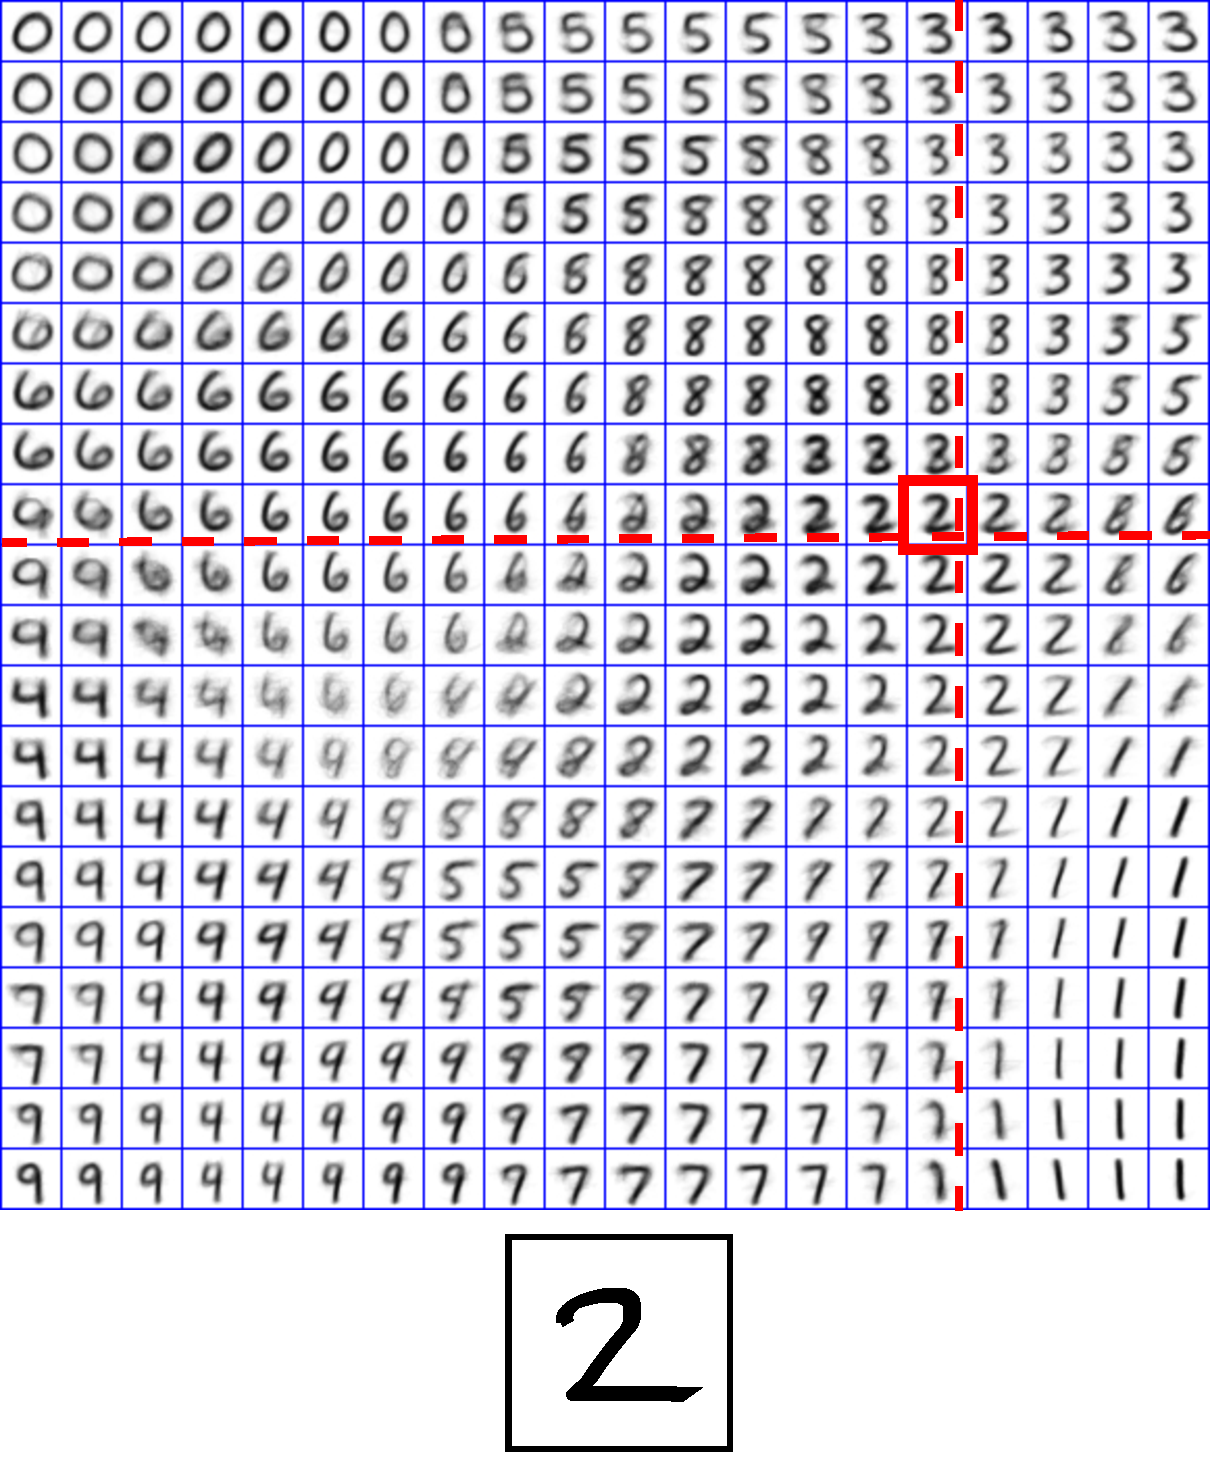
\includegraphics[width=0.3\textwidth]{digits002.pdf}
\caption{Une carte de Kohonen s'organise en zones dont les poids sont proches dans l'espace des entrées. Chaque entrée présentée à la carte peut alors être représentée par la valeur de la position du BMU correspondant dans la carte. Les entrées sont projetées sur le carré $[0,1] \times [0,1]$.}
\end{figure}

}
%\section{Travaux préliminaires sur les architectures de cartes de Kohonen}
\section{Modèle CxSOM}

Le but de cette thèse est de proposer un modèle permettant d'associer des cartes auto-organisatrices dans n'importe quel type d'architecture. En particulier, on cherchera à construire des architectures non-hiérarchiques de cartes, par exemple en figure~\ref{fig:archi_non_hierarchique}.

\begin{figure}
\centering
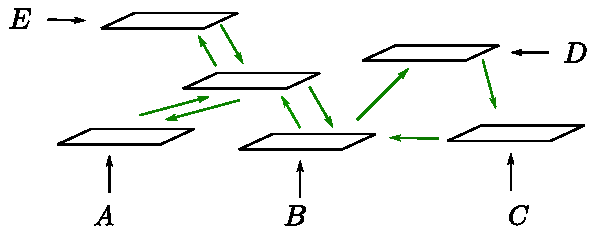
\includegraphics[width=0.6\textwidth]{architecture.pdf}
\caption{Exemple d'architecture modulaire \emph{non-hiérarchique} de cartes de Kohonen. Les entrées sont $A,B,C,D,E$ quelconques. Chaque carte peut ou non prendre une entrée ; les connexions sont réciproques ou non.}
\label{fig:archi_non_hierarchique}
\end{figure}

Dans ce modèle, l'algorithme original de Kohonen est modifié afin de connecter des cartes entre elles, et d'autoriser des connexions non-hiérarchiques.
La connexion entre une carte A et une carte B est réalisée lorsque la carte B prend comme entrée la position du Best Matching Unit de A. 
Considérons G, le graphe de connexions des cartes. Ce graphe est \emph{orienté} et les \emph{boucles} sont autorisées. C'est ce qu'on appelera \emph{architecture non-hiérarchique} de cartes, par opposition à des architectures hiérarchiques dans lesquelles le BMU d'une carte A est donné en entrée d'une carte B de façon unidirectionnelle. 

Chaque carte aura ainsi plusieurs entrées : une entrée \emph{externes} dans un espace d'entrée, facultative, et $k$ entrées \emph{contextuelles} qui sont les positions des BMUs des cartes qui lui sont connectées. Par ailleurs, la recherche du BMU doit être modifiée par rapport à l'originale : les rétroactions entre les cartes sont autorisées, la position du BMU de la carte A va donc influencer la position du BMU de la carte B, lequel modifie à nouveau le BMU de la carte A, etc. 
Notre algorithme implémente donc deux modifications principales par rapport à l'algorithme d'apprentissage d'une carte de Kohonen classique: 
\begin{itemize}
\item Les cartes possèdent plusieurs entrées, externes et contextuelles; les entrées contextuelles sont les positions des BMUs d'autres cartes. Le calcul de l'activité est donc modifié afin de prendre en compte ces différentes couches d'entrées.
\item La recherche du BMU est modifiée afin de gérer les rétroactions entre cartes.
\end{itemize}

La description du modèle CxSOM est détaillée en figure~\ref{fig:one_map}, dans un cas ou une carte reçoit deux connexions, et l'algorithme explicité en~\ref{algo:cxsom}.


\subsection{Gestion des entrées externes et contextuelles}

A un pas d'apprentissage $t$, une carte $M$ reçoit en entrée une entrée \emph{externe} notée $\inpx_t$ et $K$ entrées \emph{contextuelles} notées $\inpc_{0t},\cdots,\inpc_{Kt}$, qui sont les positions des BMU $\bmu$ des cartes qui lui sont connectées. La carte possède donc $k+1$ couches de poids. $\w_e$ correspond à l'entrée externe et $\w_{c0}, \cdots, \w_{cK}$ aux entrées contextuelles. On calcule une activité séparément sur chaque couche de poids selon la formule suivante : 
\begin{equation}
\label{eq:activite}
a(p,x) = \exp(\frac{(\w(p)-x)^2}{2\sigma^2} \; x = \inpx_t\; \text{ou}\; \inpc_{kt}, \; \w = \w_e \;\text{ou}\; \w_{ck}
\end{equation}
Les activités contextuelles sont moyennées en une activité $a_c(p,\mathbf{\inpc}_t)$, avec $\mathbf{\inpc_t} = (\inpc_{0t}, \cdots, \inpc{Kt})$. 
Les activités externes et contextuelles sont enfin fusionnées en une activité globale:
\begin{equation}
\label{eq:global_act}
a_g(p,\inpx_t,\mathbf{\inpc_t}) = \sqrt{a_e(p,\inpx_t)(\beta a_e(p,\inpx_t) + (1-\beta) a_c(p, \mathbf{\inpc_t})}
\end{equation}

Une convolution est appliquée sur cette activité globale. Cela évite les effets de plateau. Seule l'activation globale est considérée lors du calcul du BMU par relaxation, décrit en partie suivante. 

\subsection{Calcul du BMU par relaxation}

Contrairement à une carte simple, on ne peut pas calculer tous les BMUs de l'architecture en prenant l'argmax de $a_g$ dans chaque carte. A cause des influences mutuelles entre cartes, calculer le BMU d'une des cartes modifie les entrées des autres cartes de l'architecture, et donc leur BMU. Cette recherche est donc réalisée par un processus dynamique que l'on appelera \emph{relaxation}, menant à un consensus entre cartes : on cherche le point, s'il existe, où chaque BMU maximise l'activité globale de chaque carte.

Le processus de relaxation est donc une boucle imbriquée dans un pas d'apprentissage de l'architecture, indexée par $\tau$. Notons $\bmu\m[i]$ la position du BMU de la carte $i$, et $\mathbf{\bmu} = (\bmu\m[0], \cdots , \bmu\m[n])$, avec $n$ le nombre de cartes de l'architecture.
Au début d'un pas d'apprentissage, chaque carte est nourrie avec une entrée externe $\inpx^i_t$, et les activités externes $a_e^i(\inpx^i_t,p)$ de chaque carte peuvent être calculées.
La recherche du BMU suit le processus de relaxation suivant : 
\begin{enumerate}
\item Dans chaque carte $i$, la position $\bmu^i$ est initialisée à $\argmax_p(a_e^i(\inpx^i_t,p)$. Les entrées contextuelles sont alors initialisées en prenant le BMU correspondant aux connexions de l'architecture.
\item Tant que toutes les positions $\bmu^i$ ne sont pas stables, 
	\begin{enumerate}
	\item Dans chaque carte $i$, calculer les activités contextuelles et globales, définissant ainsi $p^{\star i} = \argmax_p(a_g(p,\mathbf{\inpc^i},\inpx^i)$
	\item Déplacer $\bmu^i$ vers $p^{\star i}$ : $\bmu^i \leftarrow \bmu^i \pm \Delta$ si $\lvert \bmu^i - p^{\star i} \rvert \geq \Delta$, $\bmu^i \leftarrow p^{\star i}$ sinon
	\end{enumerate}
	
\item Le BMU de chaque carte est pris comme la valeur finale stable de ce processus dynamique. Cette valeur est utilisée pour les mise a jour des poids.
\end{enumerate}

Il peut arriver que les positions se stabilisent sur un cycle limite. Dans ce cas, on arrêtera la relaxation arbitrairement; ce phénomène étant ponctuel, il n'influence pas l'apprentissage. Les paramètres des cartes de l'architecture sont choisis pour éviter de telles situations.

\begin{figure}
\centering
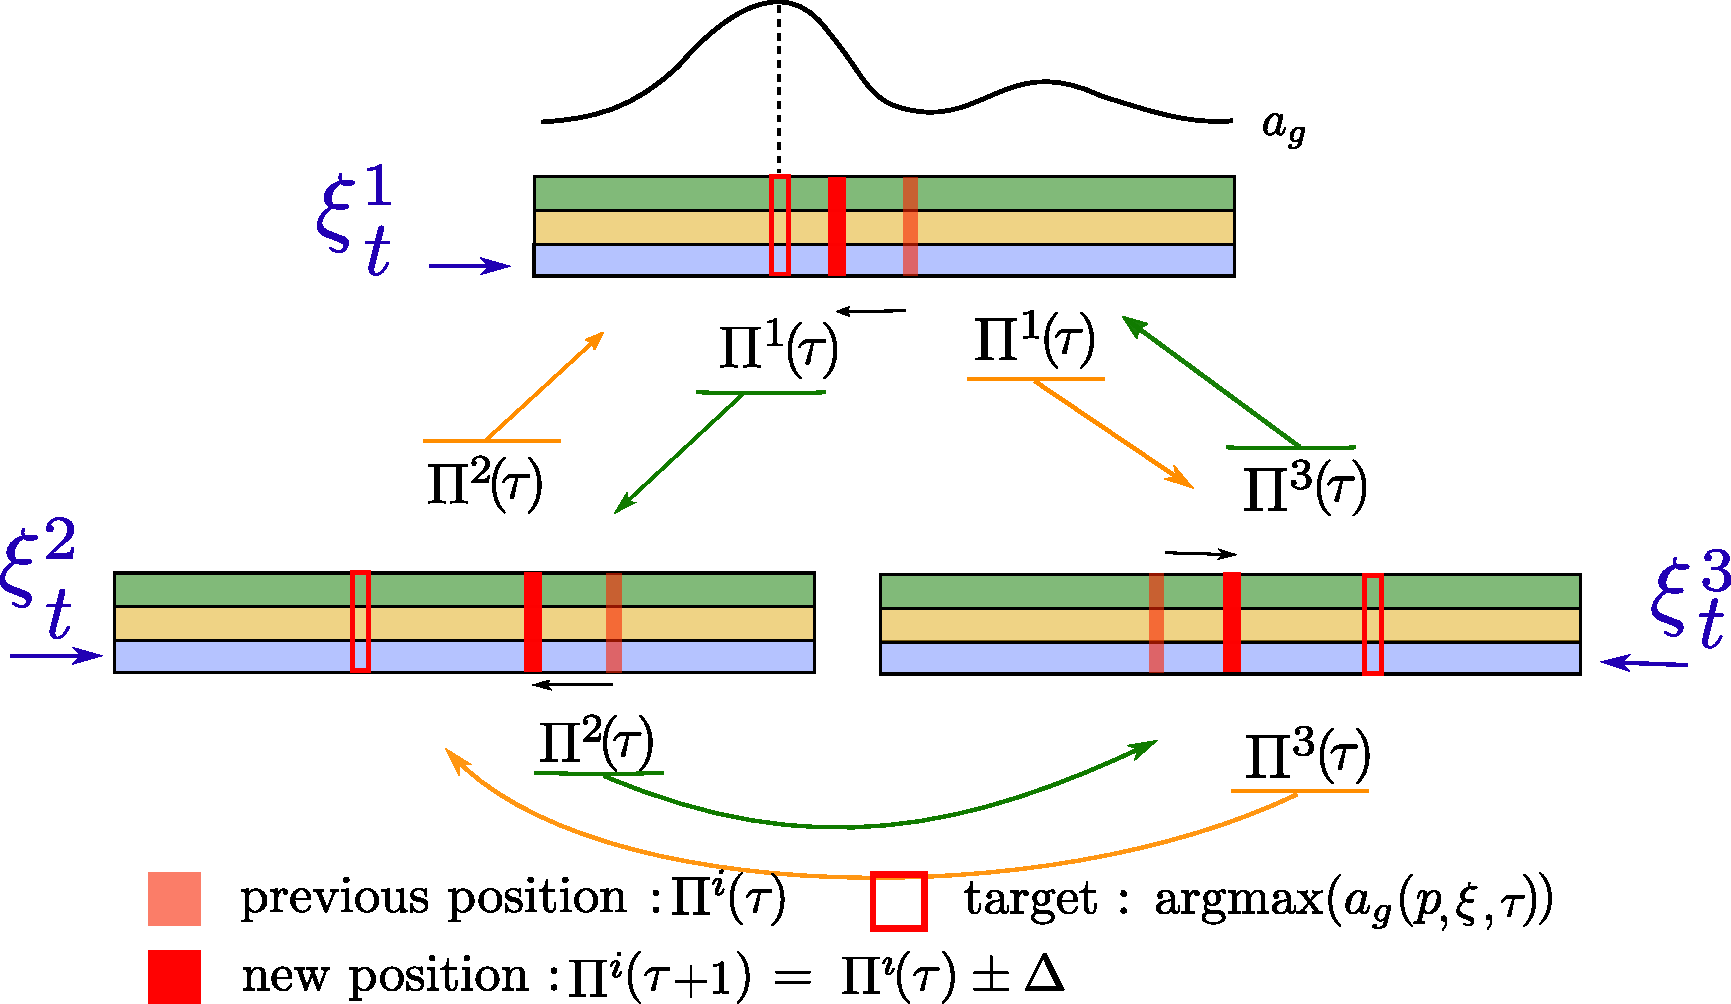
\includegraphics[width=0.6\textwidth]{relaxation.pdf}
\label{fig:relax}
\caption{description d'une étape de la relaxation dans l'architecture, aboutissant à un consensus entre cartes. Au sein d'une même itération $t$, les position des BMU $\bmu$ sont légèrement déplacées jusqu'à ce que toutes les positions $\bmu$ des cartes de l'architecture soient stable. Ces positions maximisent collectivement les activités globales de chaque carte. }
\end{figure}

\begin{figure}
\centering
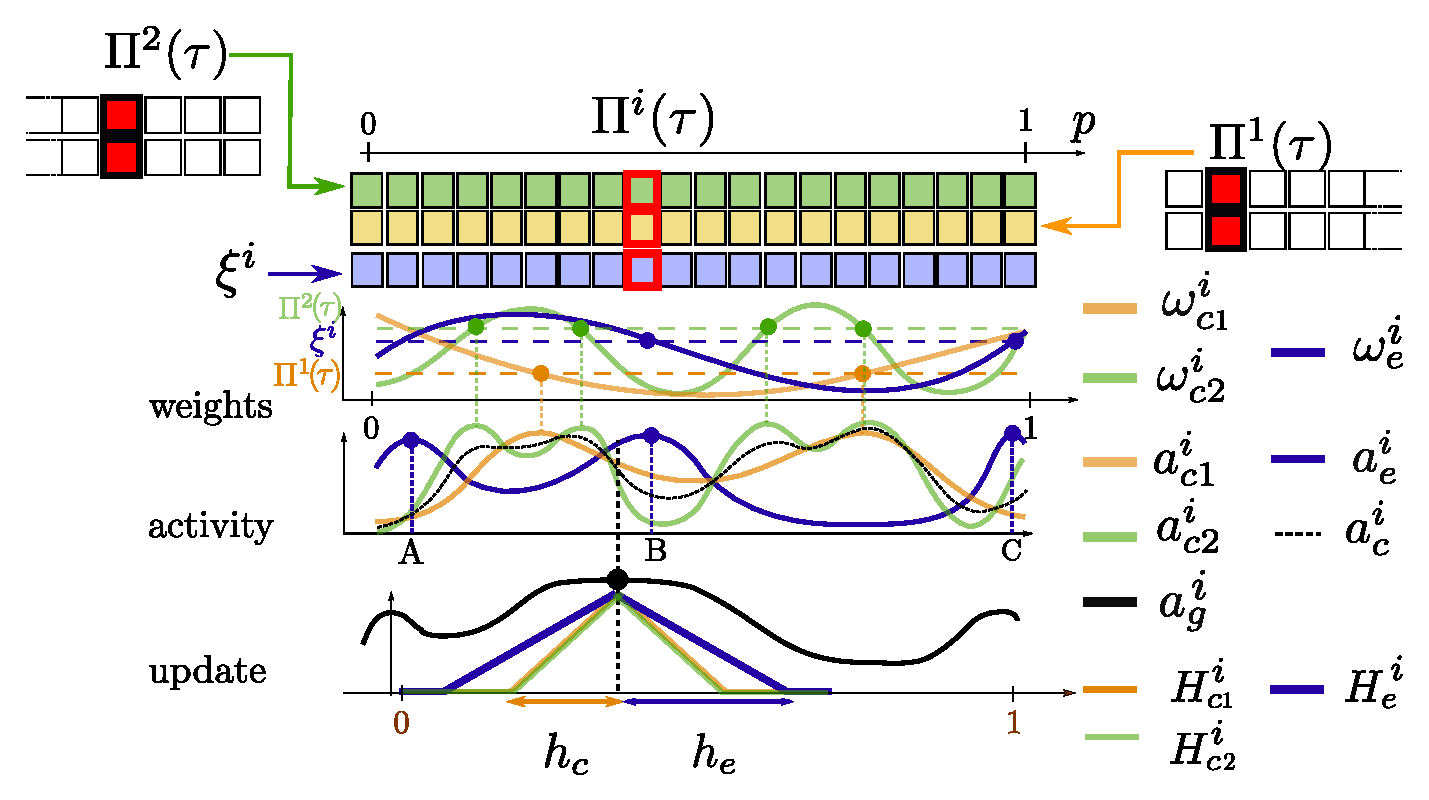
\includegraphics[width=0.8\textwidth]{one_map.pdf}
\caption{Description d'une carte au sein d'une architecture CxSOM. La carte recoit deux connexions de cartes voisines, et possède donc deux couches contextuelles}
\label{fig:one_map}
\end{figure}

\subsection{Mise à jour des poids}

Les poids sont mis à jour par rapport à leurs entrées respectives suivant l'équation \ref{eq:update}. Le BMU d'une carte est ainsi commun à toutes les couches. Les rayons de voisinage $h_e$ et $h_c$ ont des valeurs différentes ; celles-ci seront détaillée en partie suivante. 

\subsection{Résumé : Algorithme général}






\chapter{Construction d'une architecture modulaire de cartes auto-organisatrices}
\graphicspath{{03-Algorithme/}}
Le but de cette thèse est de proposer les bases d'un modèles permettant d'associer des cartes auto-organisatrices dans un cadre général. 


\section{Description de l'algorithme}

\begin{figure}
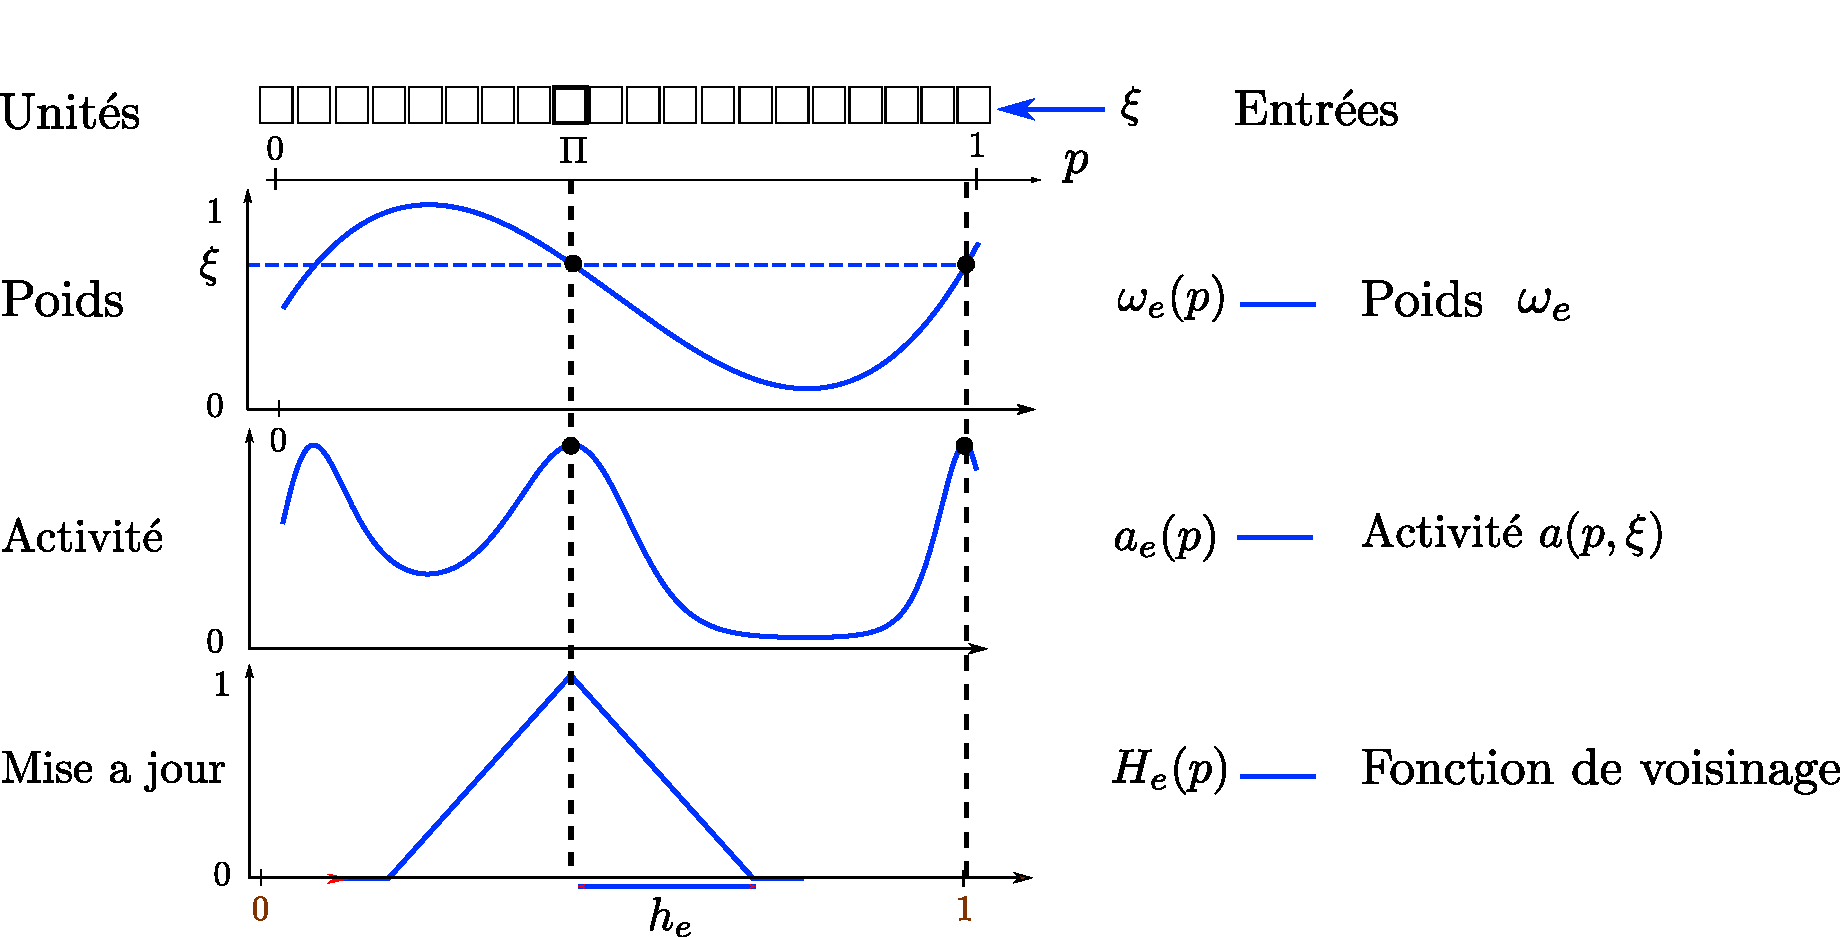
\includegraphics[width=\textwidth]{one_map_one_layer.pdf}
\caption{Notation utilisées dans une carte de Kohonen en 1 dimension}
\label{fig:one_map_not}
\end{figure}


\begin{figure}
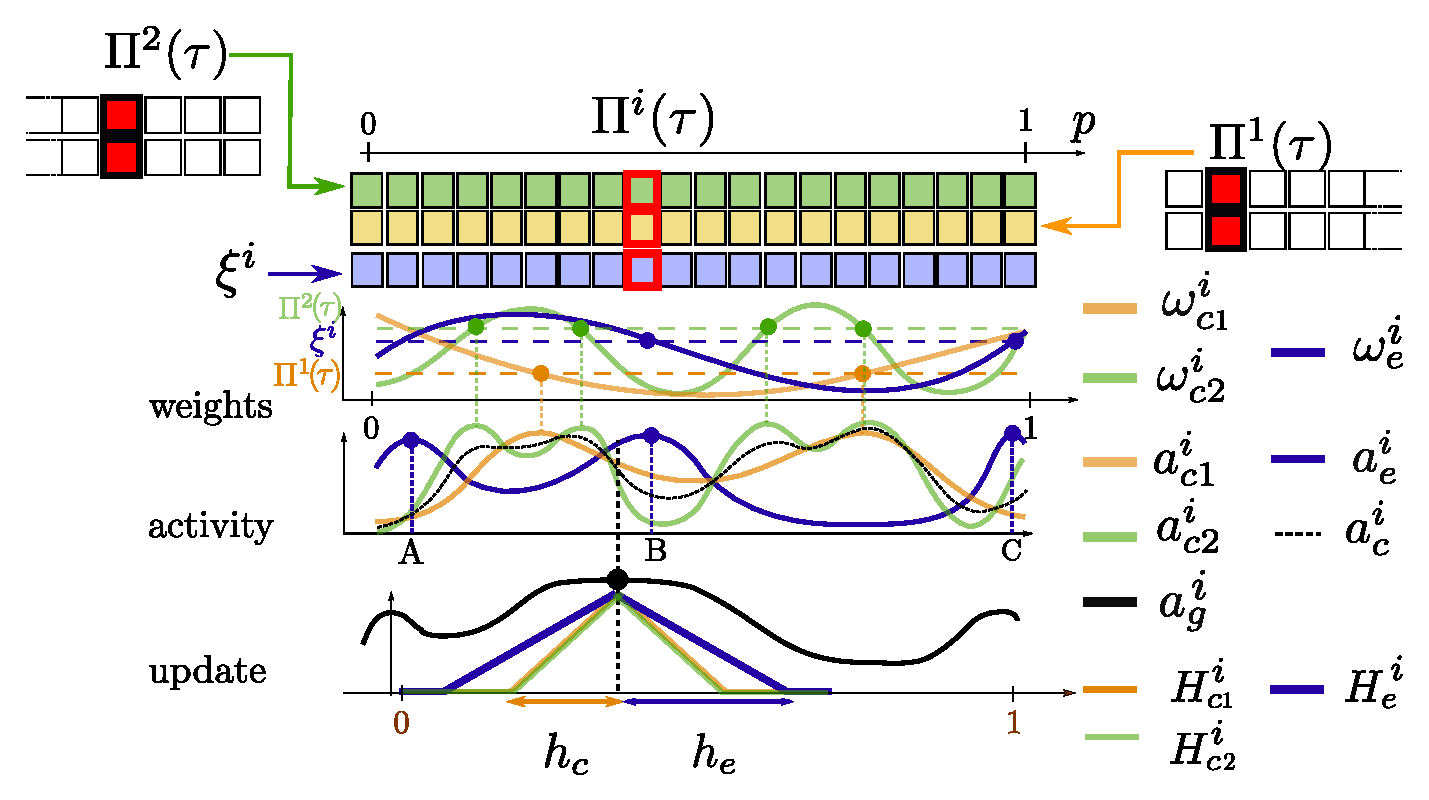
\includegraphics[width=\textwidth]{one_map.pdf}
\caption{Description d'une carte au sein d'une architecture CxSOM, avec une seule connexion.}
\label{fig:one_map}
\end{figure}


\section{Choix des paramètres}

\subsection{Influence des rayons de voisinage}

\subsection{Influence des autres paramètres}

\subsection{Compatibilité en 2D}

\section{Analyse de la relaxation}

L'apprentissage conjoint des cartes repose sur la relaxation au sein d'une itération. On cherche donc à vérifier si la relaxation converge vers une valeur quelle que soit l'entrée, et si elle est pertinente en large dimension avec de nombreuses cartes.

\subsection{Analyse expérimentale}

\subsection{Champs de BMU}

\subsection{Limitations et possibilités en grande dimension}

\section{Implémentation}
L'histoire de la recherche de consensus dans le graphe de cartes, permet que ce soit vraiment décentralisé
\chapter{Expériences : analyse provisoire et liste}
\graphicspath{{04-Analyse/}}

Cette section présente les différentes expériences réalisées afin de mieux comprendre l'architecture CxSOM. C'est une section provisoire, elle permet de mettre en relation les expériences afin d'ensuite tirer des conclusions claires a propos de l'architetecture CxSOM.
En utilisant les indicateurs et tracés présentés dans le chapitre précédent, nous détaillons dans cette partie les résltats obtenus et les pistes d'interprétation.

Les jeux de données présentés aux cartes de l'architecture sont des nuages de points en deux ou trois dimensions, tirés selon une distribution.
Les données d'entrée à l'architecture de carte seront notées $X$,$Y$,$Z$, sauf mention contraire. Ces trois valeurs sont scalaires, sont les coordonnées d'un point du nuage de point, et correspondent chacune à l'entrée d'une des cartes de l'architecture.

Dans cette version, les notations ne sont pas encore homogènes: l'autrice s'en excuse d'avance. Notez donc que : 
les modalités $X\m{i}$ sont ici notées $I^i$. L'entrée $I^i$ est toujours assignée à la carte $M^i$. Lorsqu'on utilise la variable $M^i$, il s'agit de la position du BMU $\bmu\m{i}$.

\section{Entrées sur un cercle}

Une architecture de deux cartes, connectées mutuellement, est l'exemple le plus simple d'architecture CxSOM. Son étude permet de dégager des comportements facilement représentables d'un point de vue graphique et ayant peu de liberté possible. 


\subsection{Cercle 2 dimensions}
Prenons en entrée $(X,Y)$ situé sur n cercle de centre 0.5 et de rayon 0.5, tel que $X,Y \in [0,1]$. 
Les entrées de chacune des cartes sont donc dépendantes. Nous regarderons la distribution des valeurs selon les BMU de chaque carte.

\begin{figure}[h!]
\begin{minipage}{0.33\textwidth}
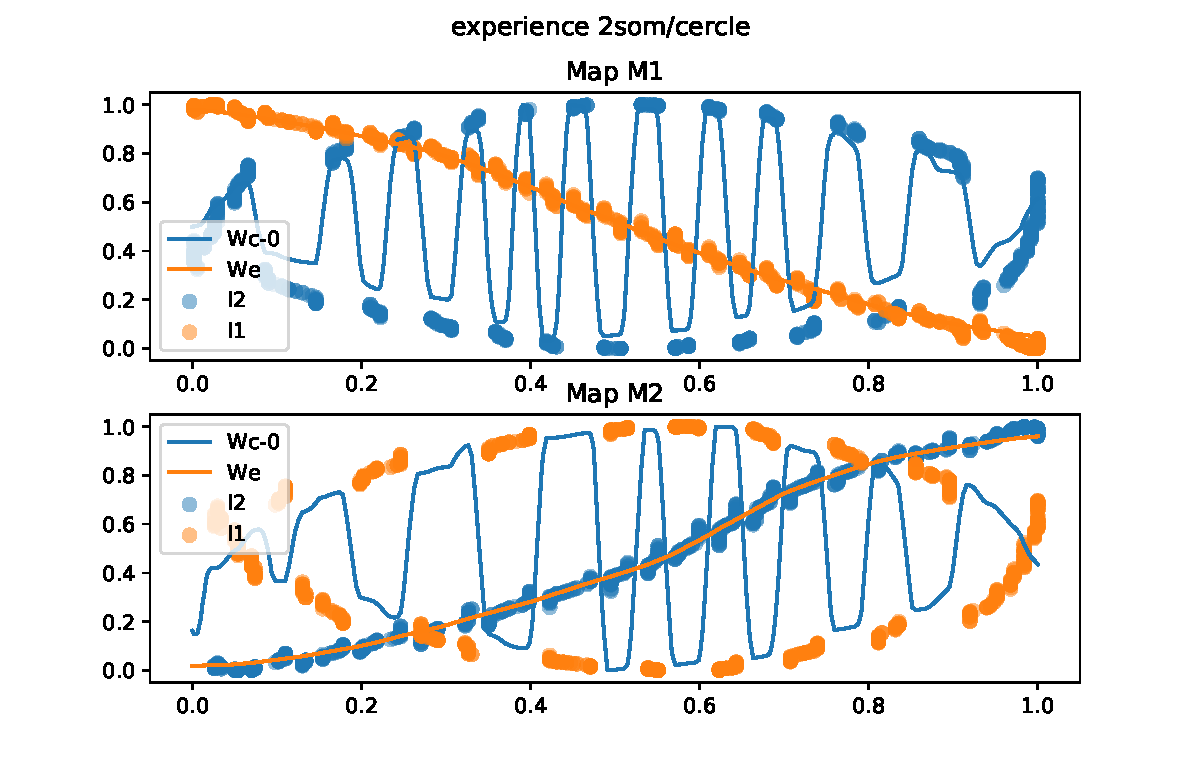
\includegraphics[width=\textwidth]{2som_cercle_w.pdf}
\end{minipage}
\begin{minipage}{0.33\textwidth}
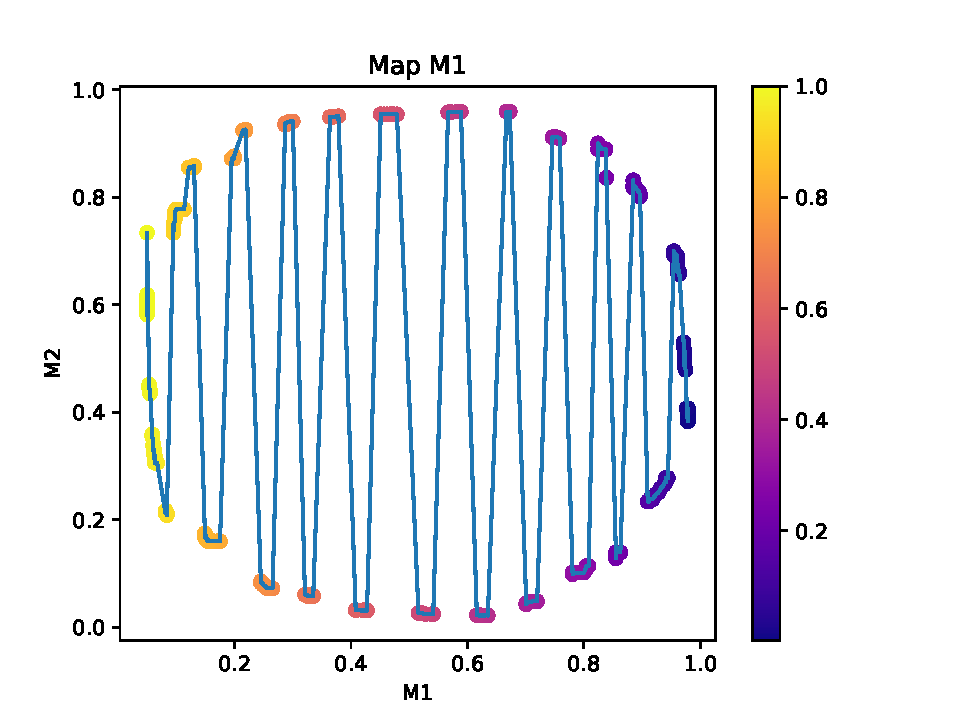
\includegraphics[width=\textwidth]{2som_cercle_d.pdf}
\end{minipage}
\begin{minipage}{0.33\textwidth}
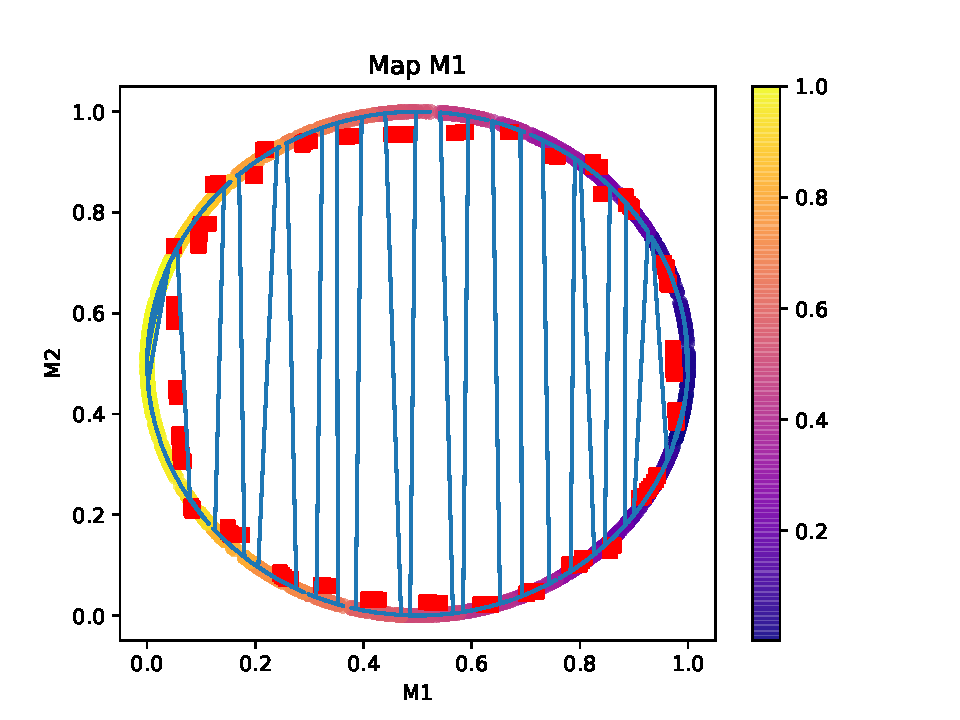
\includegraphics[width=\textwidth]{2som_cercle_din.pdf}
\end{minipage}
\label{fig:2som_square}
\caption{Tracé des poids de M1 et M2, dépliement des poids de M1 dans l'espace 2D et dépliement des entrées}
\end{figure}

\subsection{Cercle trois dimensions}

Les entrées sont $(X,Y,Z)$, trois cartes connectées mutuellement. Les entrées sont dépendantes de telle sorte à ce que connaitre l'une d'entre elle laisse 50\% d'erreur sur les deux autre, mais deux d'entre elle permettent de déterminer totalement la troisième. 

En figure~\ref{fig:3som_cercle}
\begin{figure}[h!]
\begin{minipage}{0.33\textwidth}
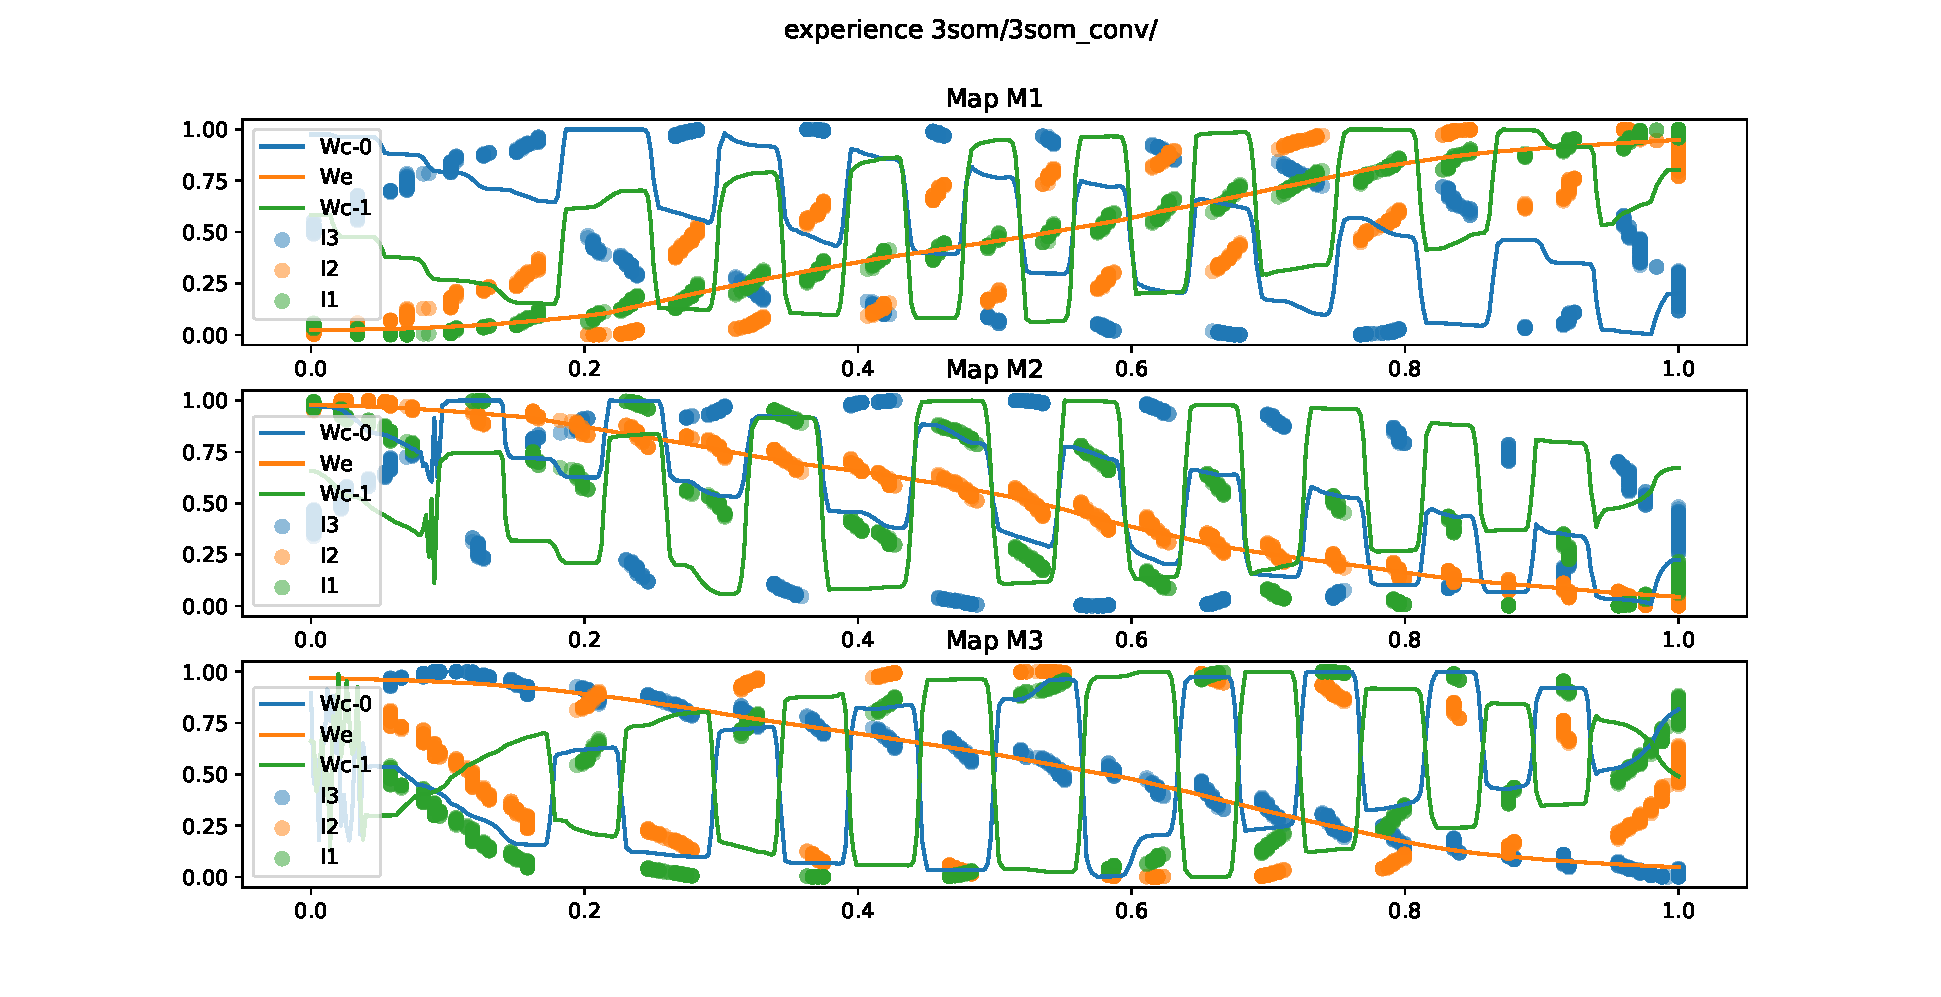
\includegraphics[width=\textwidth]{3som_cercle_w}
\end{minipage}
\begin{minipage}{0.33\textwidth}
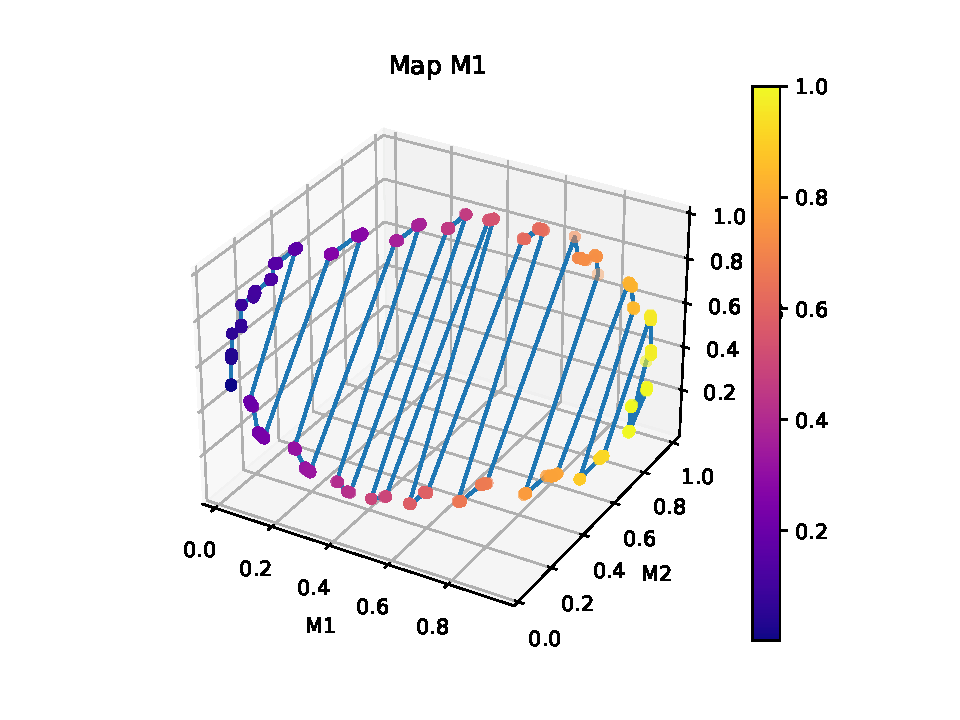
\includegraphics[width=\textwidth]{3som_cercle_dw1}
\end{minipage}
\begin{minipage}{0.33\textwidth}
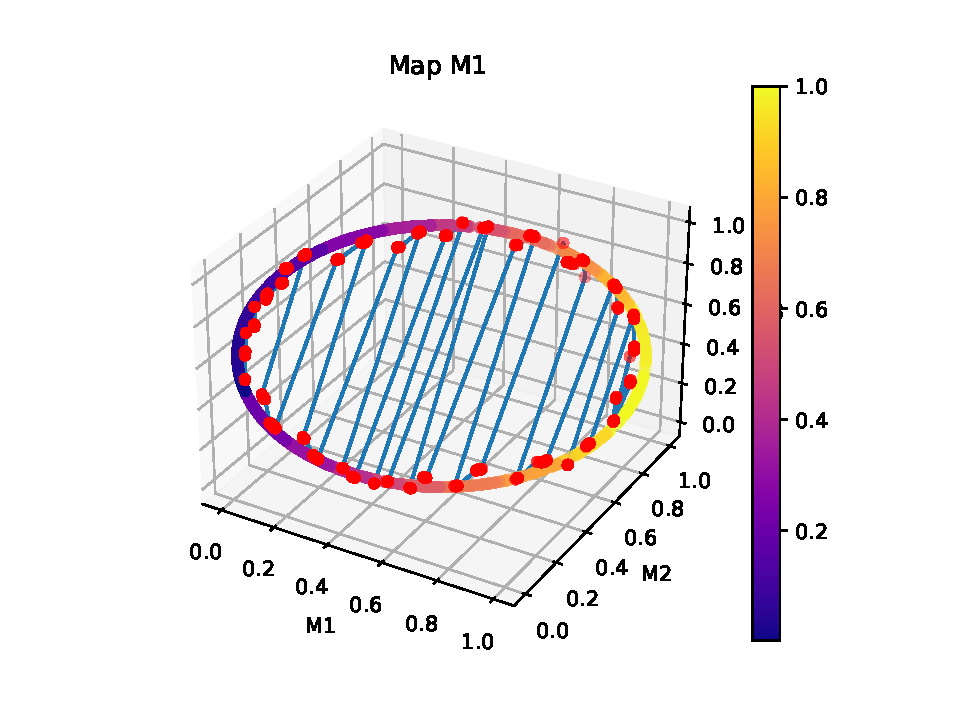
\includegraphics[width=\textwidth]{3som_cercle_din1}
\end{minipage}
\end{figure}
\begin{figure}
\centering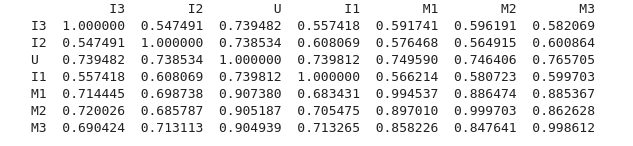
\includegraphics[width=0.8\textwidth]{3som_cercle_im}
\caption{Valeurs de $UC$ entre les différents éléments des cartes pour des entrées sur un cercle. Pour un élément $i,j$ du tableau est indiqué $UC(i|j)$ (Mi correspond à $\Pi\m{i}$. Le tableau sera mis au propre s'il est pertinent. Estimation par la méthode de Kraskov, voisinage de 7. Ce voisinage est arbitraire, il produit une variance plus grande mais biais moins important. Il faudrait refaire l'expé sur de multiple echantillons pour avoir une valeur sure. }
\label{fig:3som_cercle}
\end{figure}



\subsection{Entrées dans un anneau}

On peut, au lieu de considérer un cercle, ajouter du bruit à chaque dimension. Les entrées sont alors tirées dans un fin anneau ou tore. Dans ces conditions, le modèle peut toujours être considéré comme un cercle avec bruit. On peut donc prendre $U$ en une dimension :  
$$
 \begin{cases}
     X_t = r  \cos(U_t) + \epsilon_X\\
     Y_t = r \sin(U_t) + \epsilon_Y
    \end{cases}\,.
$$
Cenpendant, on peut aussi considérer que le modèle n'est plus réductible en une seule dimension cachée.
Il est donc intéressant de regarder comment les cartes considèrent le bruit : a-t-on toujours une quantification vectorielle du cercle, ou la carte se déplie t-elle autrement ? Autrement dit, une carte sépare t-elle le bruit de la forme des entrées ?

\begin{figure}
\centering
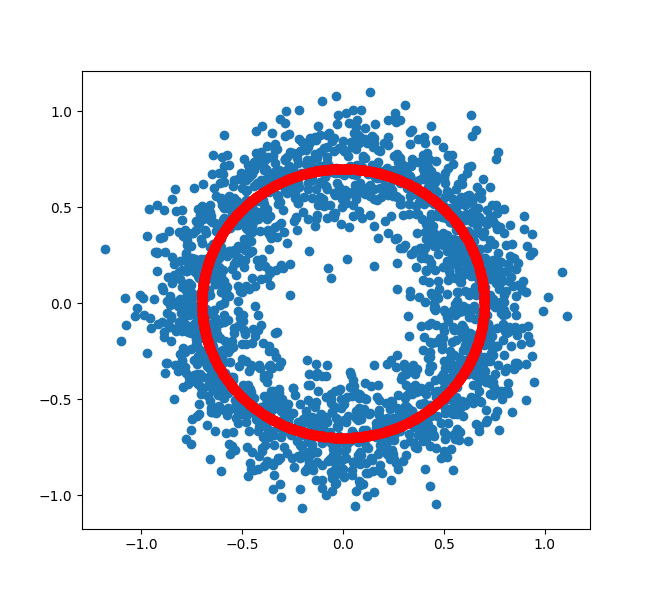
\includegraphics[width=0.4\textwidth]{inputs_anneau_cercle.png}
\caption{Entrées d'apprentissage en bleu, entrées test en rouge}
\label{fig:inputs_anneau_cercle}
\end{figure}

Pour le vérifier, on peut, à partir des poids appris sur des données bruitées, réaliser les tests sur des données non bruitée, donc un cercle, entrées présentées en figure~\ref{fig:inputs_anneau_cercle}.
Dans ce cas, la prédiction et la répartition est semblable au cas ou les cartes ont appris le cercle : la quantification est résistante au bruit, comme présenté en figure~\ref{fig:anneau_cercle}. On regardera donc par la suite le comportement des cartes sur des données non bruitées. 

\begin{figure}
\begin{minipage}{0.5\textwidth}
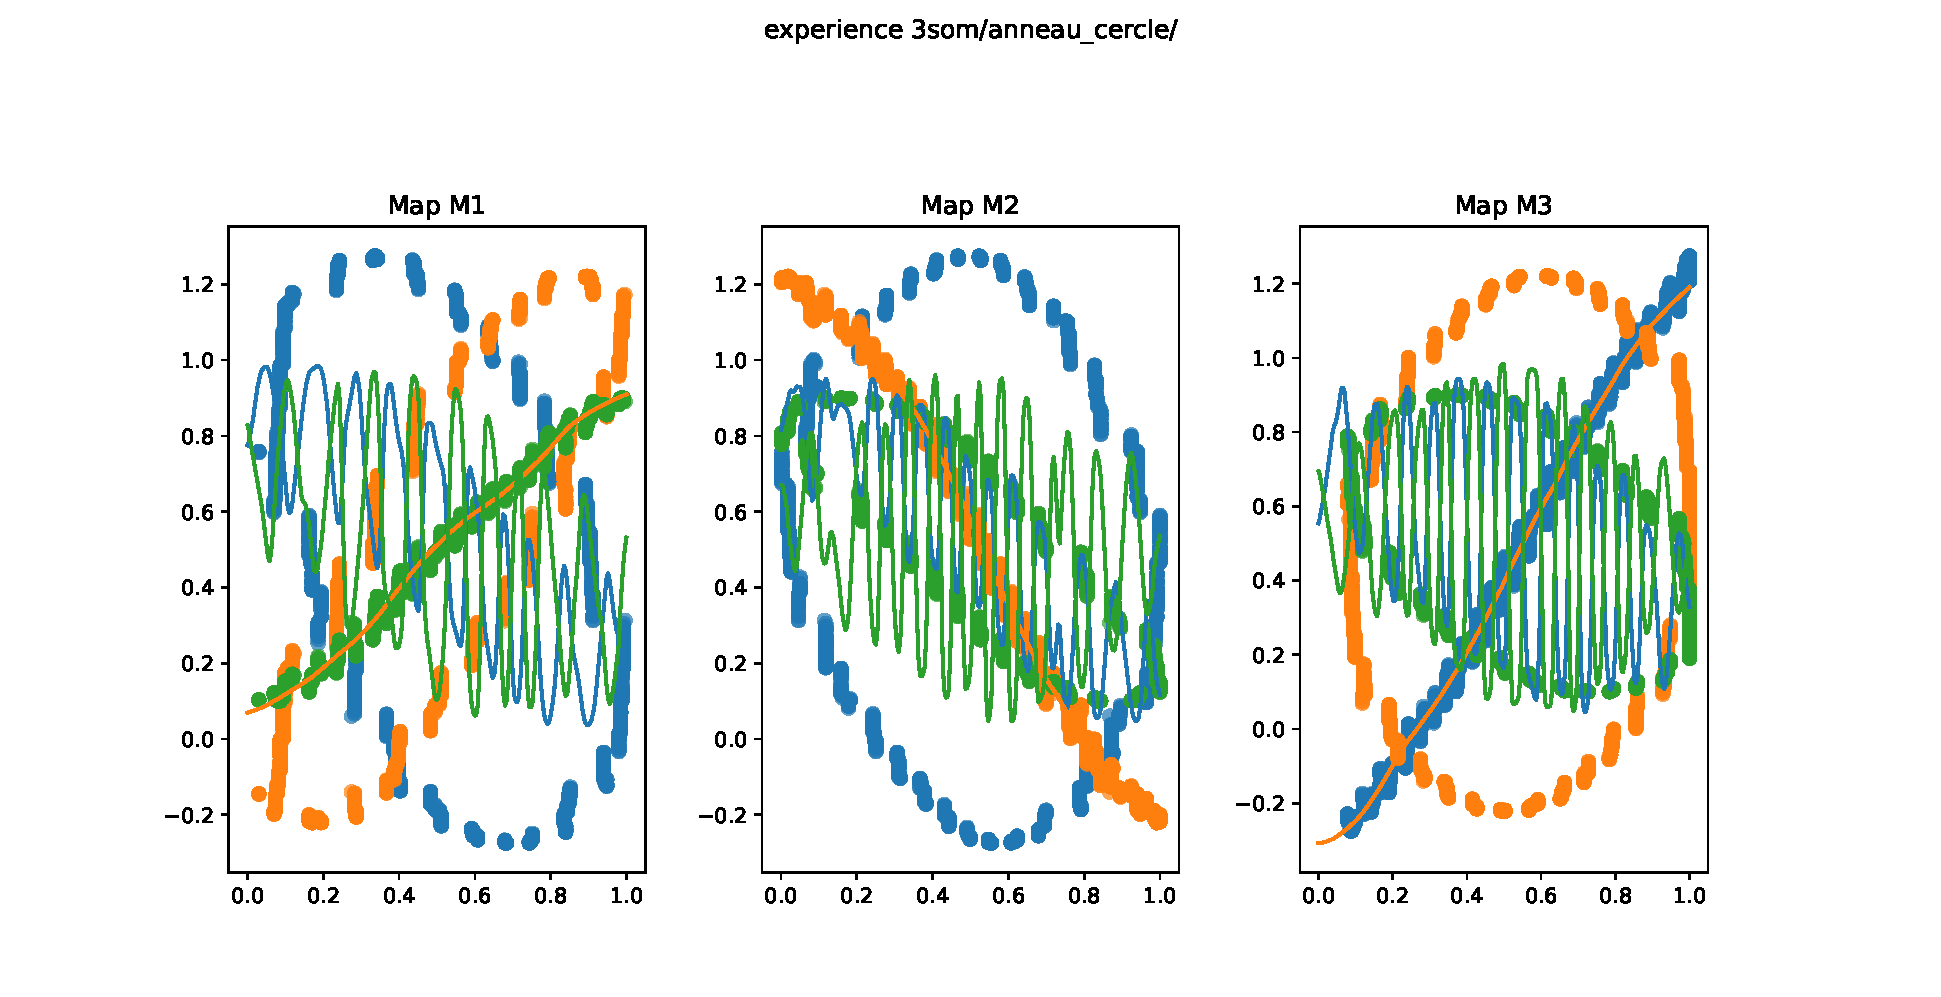
\includegraphics[width=\textwidth]{3som_anneau_cercle_w.pdf}
\end{minipage}
\begin{minipage}{0.5\textwidth}
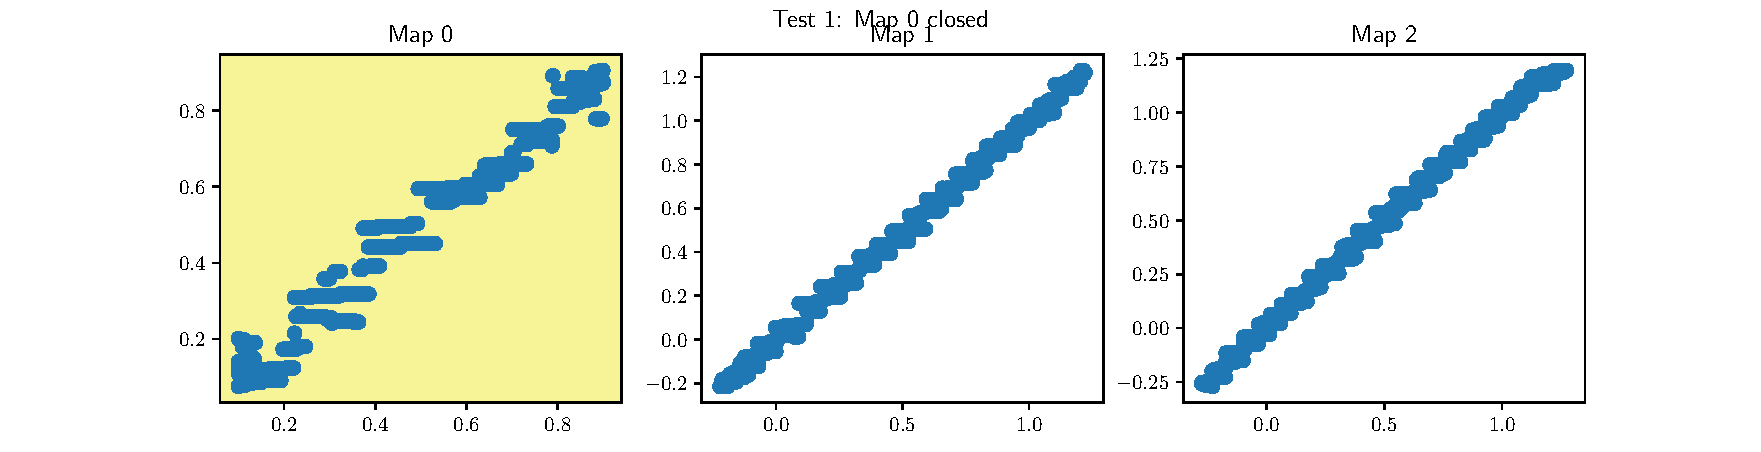
\includegraphics[width=\textwidth]{3som_anneau_cercle_pred.pdf}
\end{minipage}
\caption{L'apprentissage a été réalisé sur un cercle en 3D avec bruit, les tests sur le cercle. La répartition des entrées et poids et la prédiction est réalisée comme sur le cercle : la quantification vectorielle est résistante au bruit. }
\label{fig:anneau_cercle}
\end{figure}

\section{Entrées dans un carré}

\subsubsection{Expérience}
Prenons en entrée $(X,Y) \in [0,1]^2$, tirés selon une distribution uniforme. Les entrées de chacune des cartes sont donc indépendantes. Nous regarderons la distribution des valeurs selon les BMU de chaque carte. Cette distribution de valeurs dépendra donc uniquement de l'architecture, étant données que les entrées n'ont aucun lien entre elles. Cela nous permet de visualiser quels comportements sont uniquement issus du modèle.
 
\subsubsection{Résultats}

\begin{figure}[h!]
\begin{minipage}{0.33\textwidth}
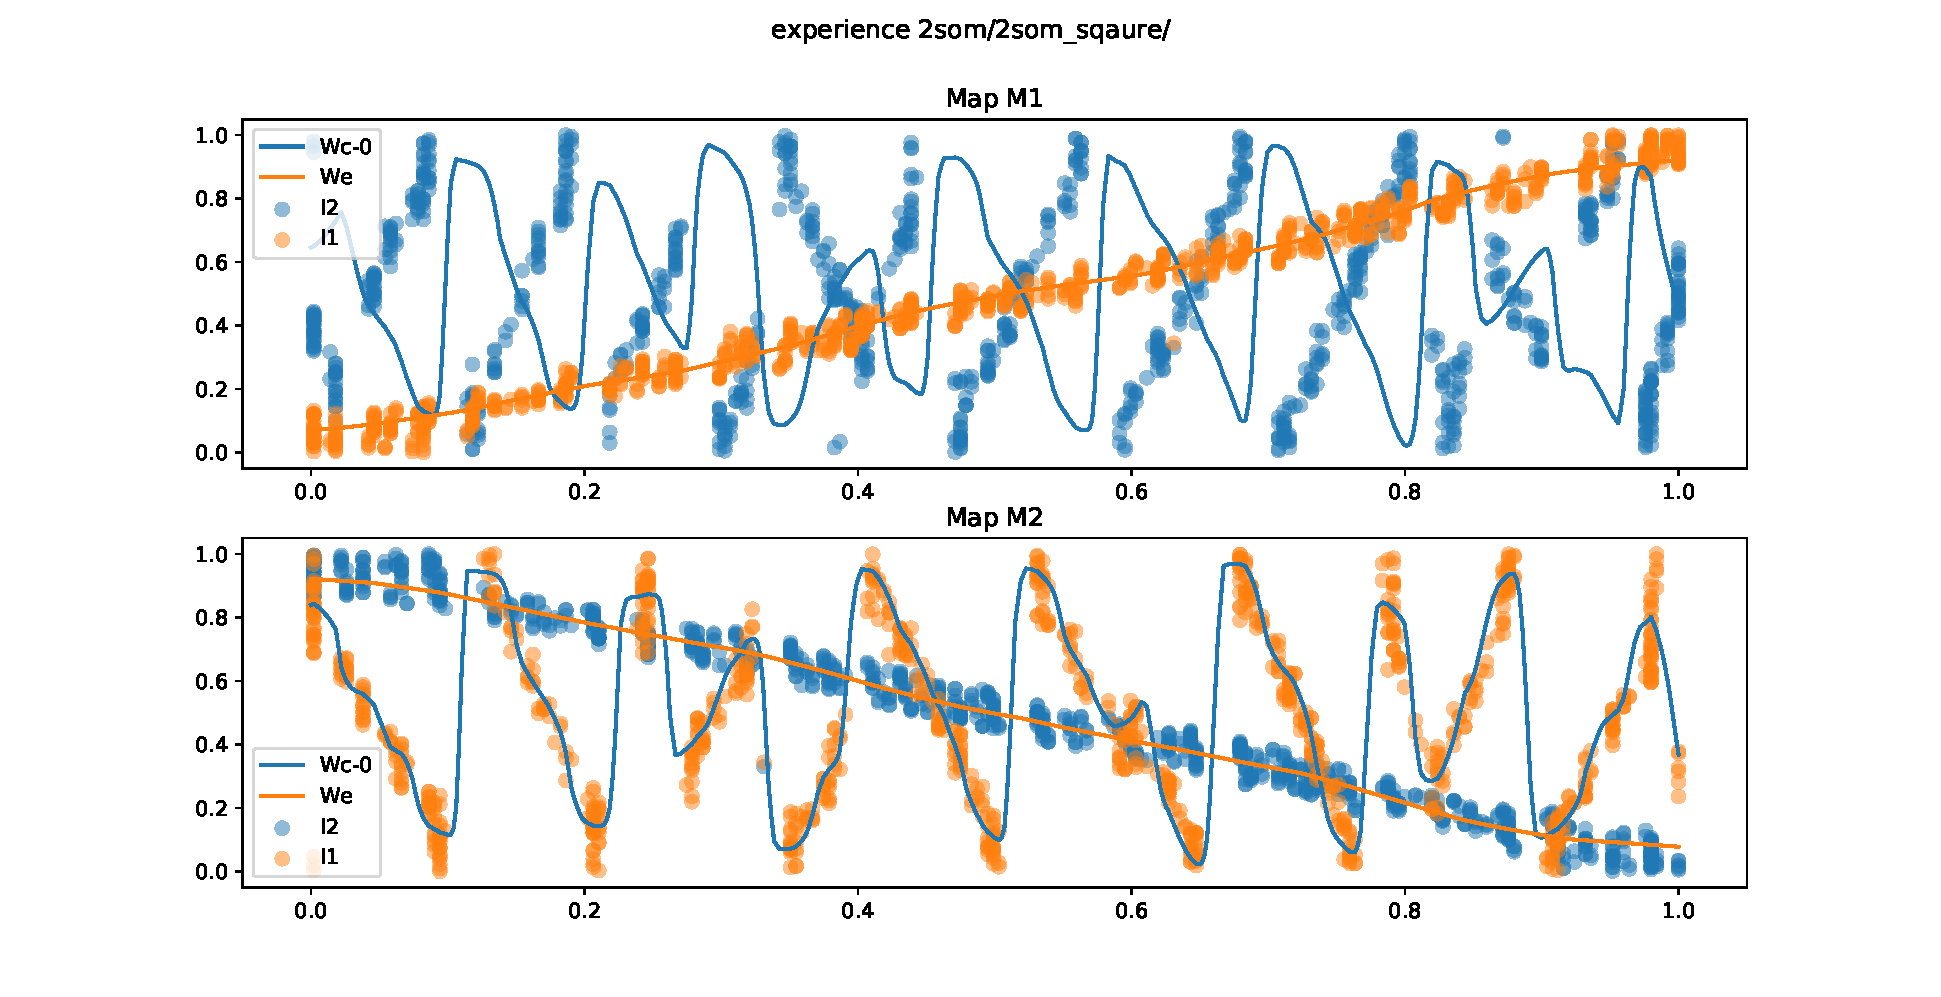
\includegraphics[width=\textwidth]{2som_square_w.pdf}
\end{minipage}
\begin{minipage}{0.33\textwidth}
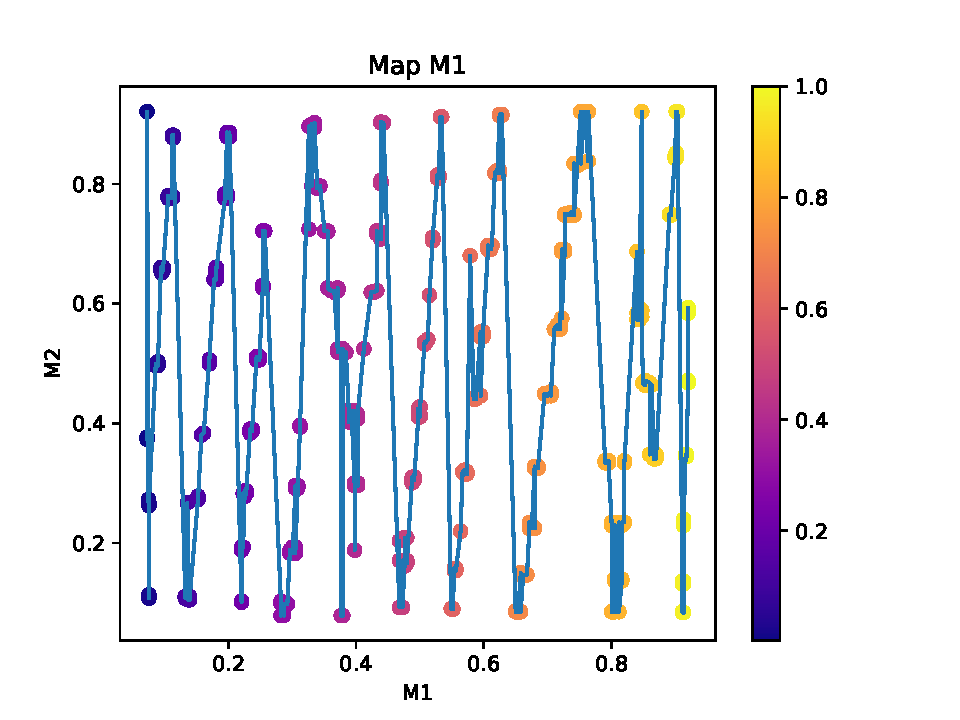
\includegraphics[width=\textwidth]{2som_square_d.pdf}
\end{minipage}
\begin{minipage}{0.33\textwidth}
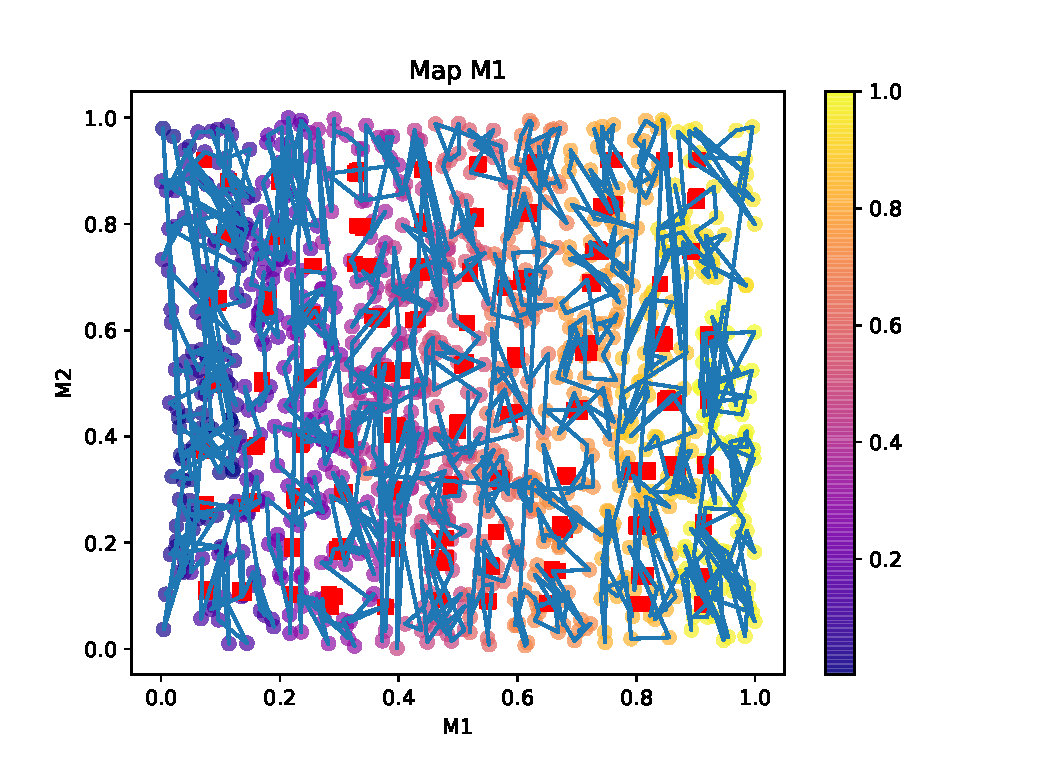
\includegraphics[width=\textwidth]{2som_square_din.pdf}
\end{minipage}
\label{fig:2som_square}
\caption{Tracé des poids de M1 et M2, dépliement des poids de M1 dans l'espace 2D et dépliement des entrées}
\end{figure}

Cette expérience montre que la disposition en vagues des cartes est un comportement lié à l'architecture et non aux données en elles même : quelles que soient les données, la carte effectuera toujours une séparation en indices primaires et secondaires. Ici, pour un X donné, on a toutes les valeurs possibles pour Y.
Cependant, les poids sont un peu différents de l'expérience avec X,Y sur un cercle : les bmus au sein d'une zone secondaire sont répartis tout le long de cette zone, alors que pour un cercle ils sont centrés dans la zone.
C'est intéressant de voir que même si seuls les poids contextuels ne nous éclairent pas trop sur le comportement des cartes, leur forme traduit quand même un aspect du modèle. 


\section{Entrées en clusters}

On considère des entrées $X$, $Y$ distribuées dans $[0,1]^2$, telles que les points sont regroupés autour de 6 centres. Autour de ces centres, les points sont tirés aléatoirement dans un cercle. On a donc des clusters de points. La distribution de $(X,Y)$ peut être considérée comme fonction des centres des clusters.  A-t-on un regroupement des points des clusters dans la carte, ou la carte se déplie t-elle sans prendre en compte les regroupement ? Nous présentons ici deux expériences, chacune prenant des entrées distribuées selon des tailles différentes de clusters autour de leurs centres, tracées en figure~\ref{fig:cluster_in}.  $U$ est ici considéré comme l'indice (entre 0 et 1) du cluster.

\begin{figure}[h!]
\begin{minipage}{0.5\textwidth}
\centering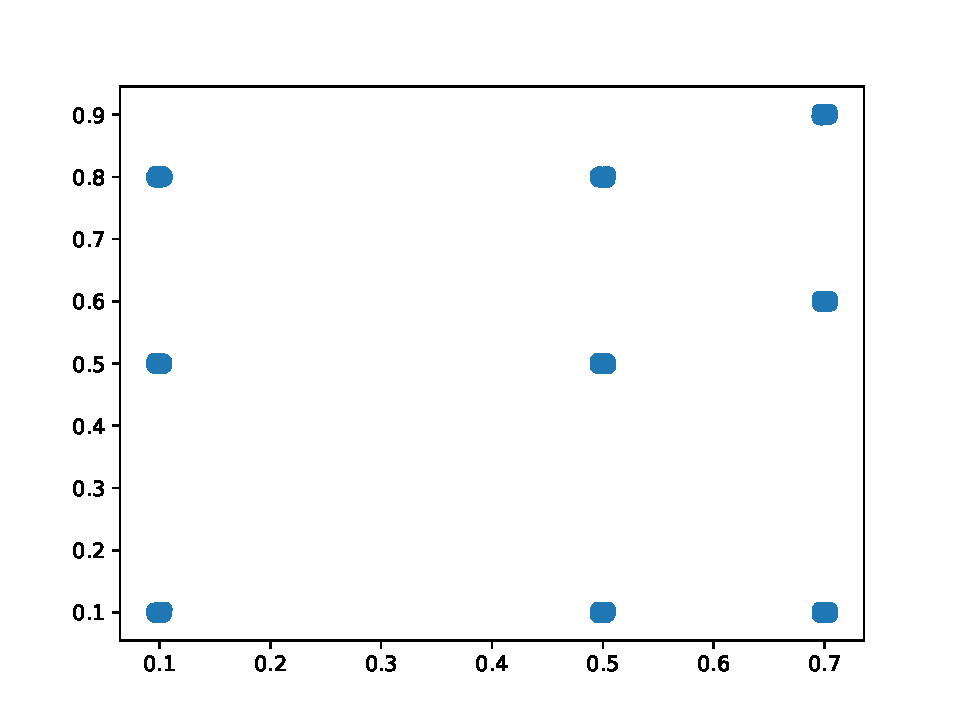
\includegraphics[width=0.7\textwidth]{2som_cluster_in}
\end{minipage}
\begin{minipage}{0.5\textwidth}
\centering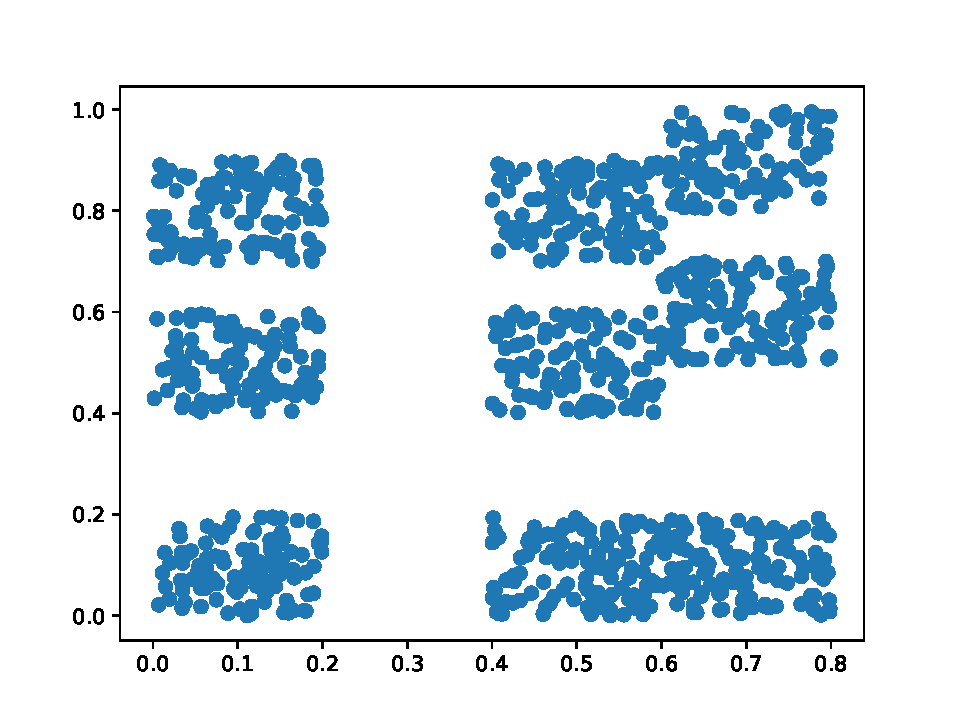
\includegraphics[width=0.7\textwidth]{2som_cluster001_in}
\end{minipage}
\caption{Entrées présentées aux cartes dans chaque expériences. A gauche, "petits" clusters, à droite, "grands" clusters}
\label{fig:cluster_in}
\end{figure}



\subsection{"petits" clusters}

\begin{figure}[h!]
\begin{minipage}{0.33\textwidth}
\centering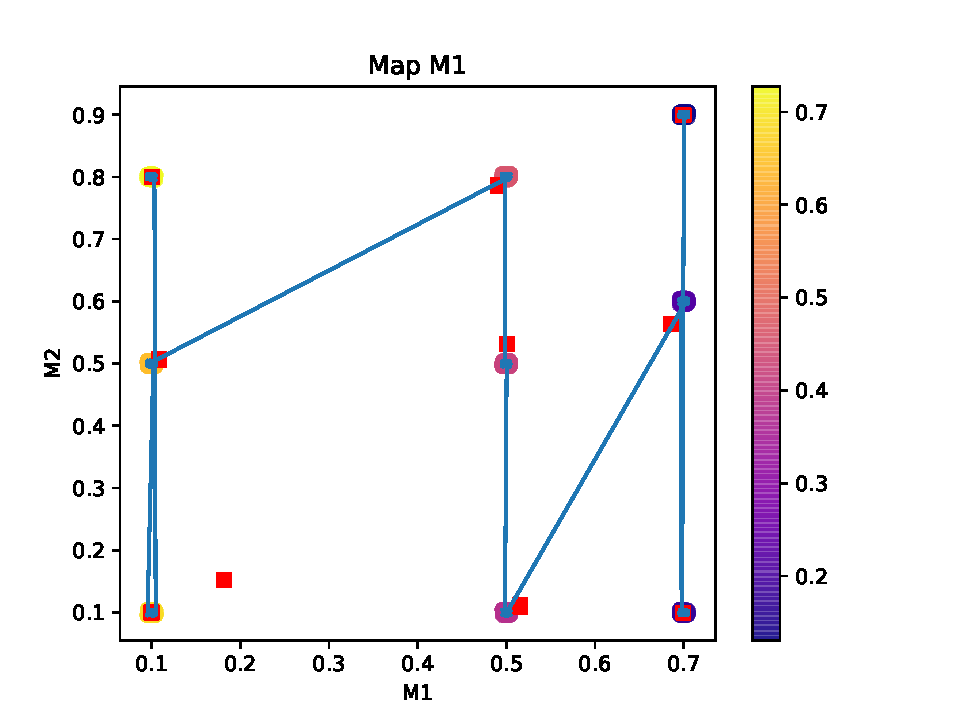
\includegraphics[width=\textwidth]{2som_cluster_din}
\end{minipage}
\begin{minipage}{0.33\textwidth}
\centering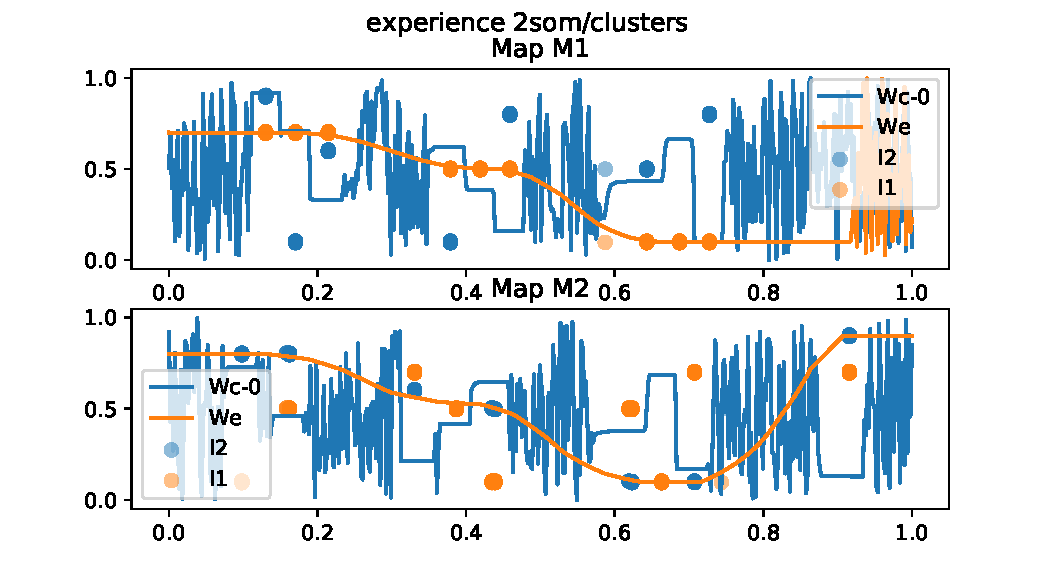
\includegraphics[width=\textwidth]{2som_cluster_w}
\end{minipage}
\begin{minipage}{0.33\textwidth}
\centering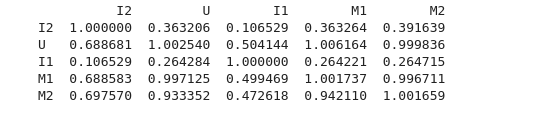
\includegraphics[width=\textwidth]{2som_clusterssmall_im.png}
\end{minipage}
\caption{Dépliement, poids et information mutuelles des cartes. }
\label{fig:cluster}
\end{figure}

La carte se déplie en suivant les clusters : un ensemble de BMU proche code pour un cluster. 

\subsection{"gros" clusters}

\begin{figure}[h!]
\begin{minipage}{0.33\textwidth}
\centering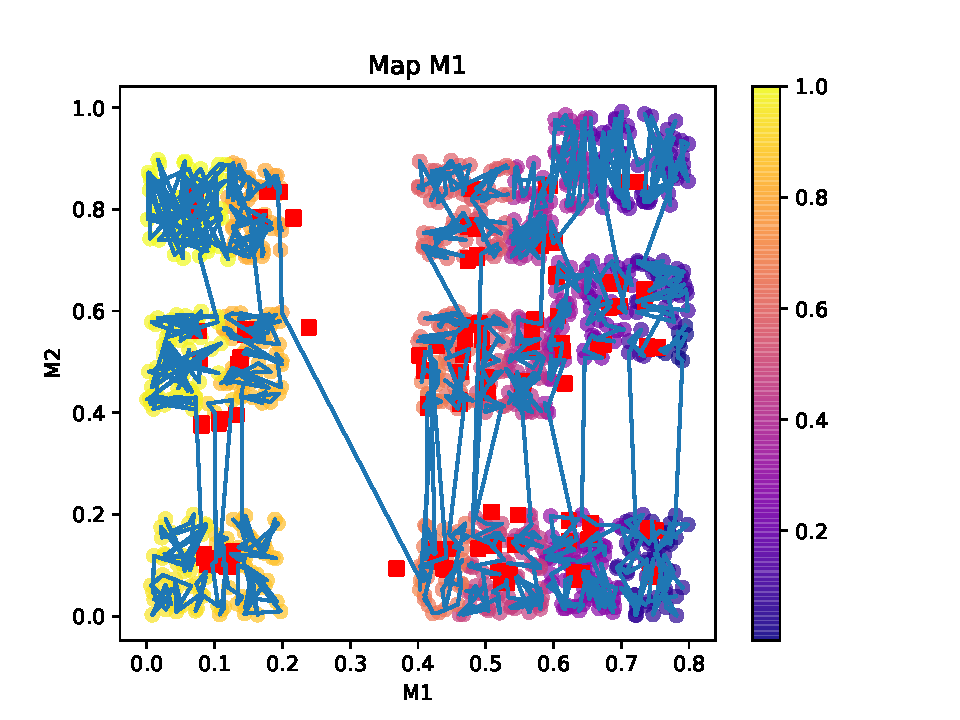
\includegraphics[width=\textwidth]{2som_cluster001_din}
\end{minipage}
\begin{minipage}{0.33\textwidth}
\centering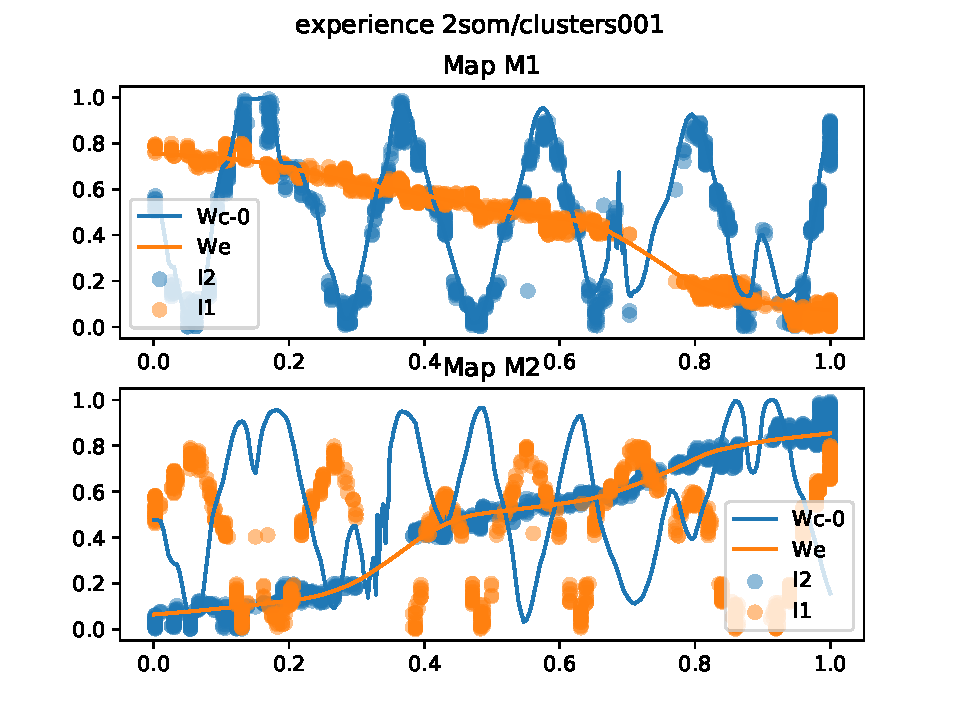
\includegraphics[width=\textwidth]{2som_cluster001_w}
\end{minipage}
\begin{minipage}{0.33\textwidth}
\end{minipage}
\caption{Dépliement, poids et information mutuelles des cartes. }
\label{fig:cluster001}
\end{figure}

La carte sépare les éléments d'un même cluster en plusieurs zones. Par contre, un ensemble de BMU code pour une partie d'un cluster, mais ne correspond  


\section{Influence de l'architecture sur des entrées}

Sur des entrées identiques, on testera différentes architectures afin d'évaluer le rôle des connexions. On utilisera toujours comme entrée dans cette section un cercle en deux ou trois dimensions. 
Comme on a vu dans les sections précédentes, l'architecture est robuste aux entrées bruitées; on utilise donc ici des entrées sans bruit. 

\subsection{Cartes intermédiaires}
mettre line 4 som, etc. 

information mutuelle dans ce cas :) comparer a la version une carte intermédiare. 
Tableau info mutuelle : faire les comparaisons. Comparaison des entrées, ce sont a peu près les mêmes donc on doit avoir les memes valeurs ok, donc ce qui nous intéresse c'est la comparaison entre M1 M2 M3 M4 etc. 

Dans cette expérience, les entrées sont $X,Y$ ou $X,Y,Z$, sur un cercle en 2D ou 3D; l'architecture est composée de 3 cartes, une prenant $X$, une prenant $X$ et une connectée aux deux autres ne prenant que les BMUs en entrée. Les cartes $X$ et $Y$ ne sont pas directement connectées. On testera l'architecture avec une et deux cartes intermédiaires pour la version 2D (figure~\ref{fig:archi_intermediaire}).
Pour la version 3D, on a une carte centrale. 

\begin{figure}[h!]

\includegraphics[width=0.7\textwidth]{archi_intermediaire.png}
\caption{Architectures avec une (1) et deux (2) cartes intermédiaires sans entrées, présentées dans cette section. }
\label{fig:archi_intermediaire}
\end{figure}

\begin{figure}[h!]
\begin{minipage}{0.5\textwidth}
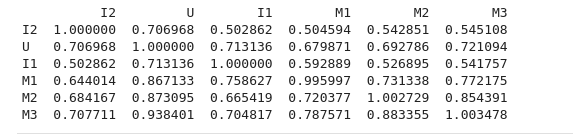
\includegraphics[width=\textwidth]{2som_star_im.png}
\end{minipage}
\begin{minipage}{0.5\textwidth}
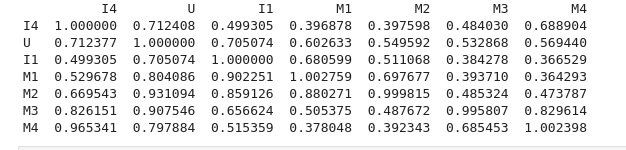
\includegraphics[width=\textwidth]{2som_line4_im.png}
\end{minipage}
\caption{coefficients d'incertitude entre les éléments des cartes, pour l'architecture (1)(gauche) et (2)(droite). Le nombre de voisins utilisés pour l'estimation est 10. L'estimation est réalisée sur 1000 échantillons. $I1$ est l'entrée de la carte $M1$ et correspond à $X$,  $I2$ ou $I4$ est l'entrée de la carte 2 ou 4 et correspond à $Y$. }
\end{figure}



\begin{figure}[h!]
\begin{minipage}{0.5\textwidth}
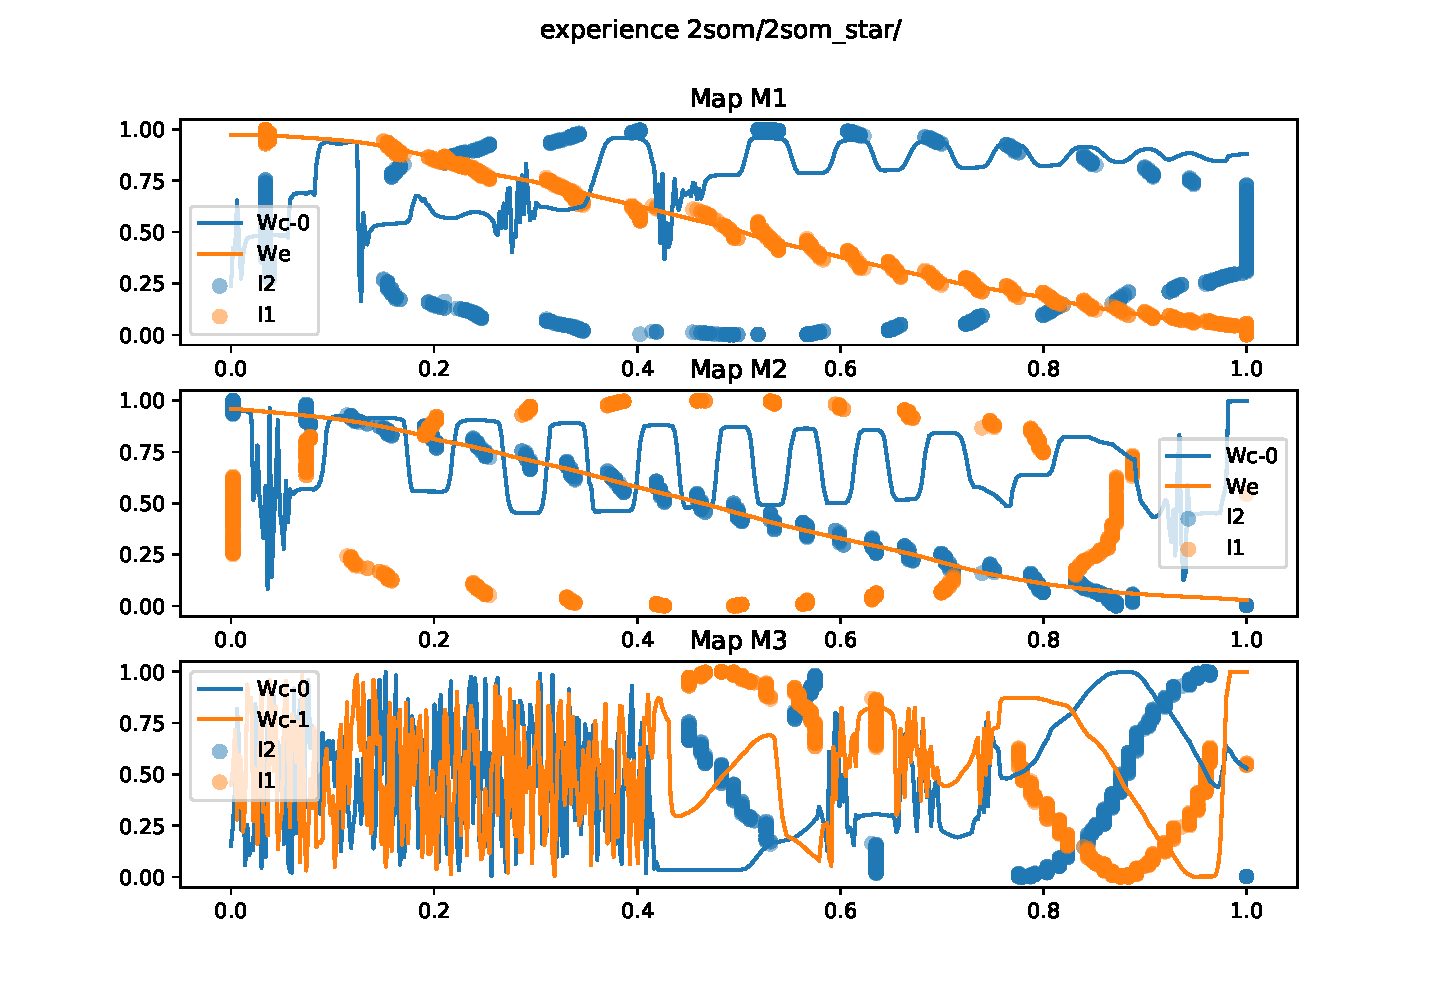
\includegraphics[width=\textwidth]{2som_star_w.pdf}
\end{minipage}
\begin{minipage}{0.5\textwidth}
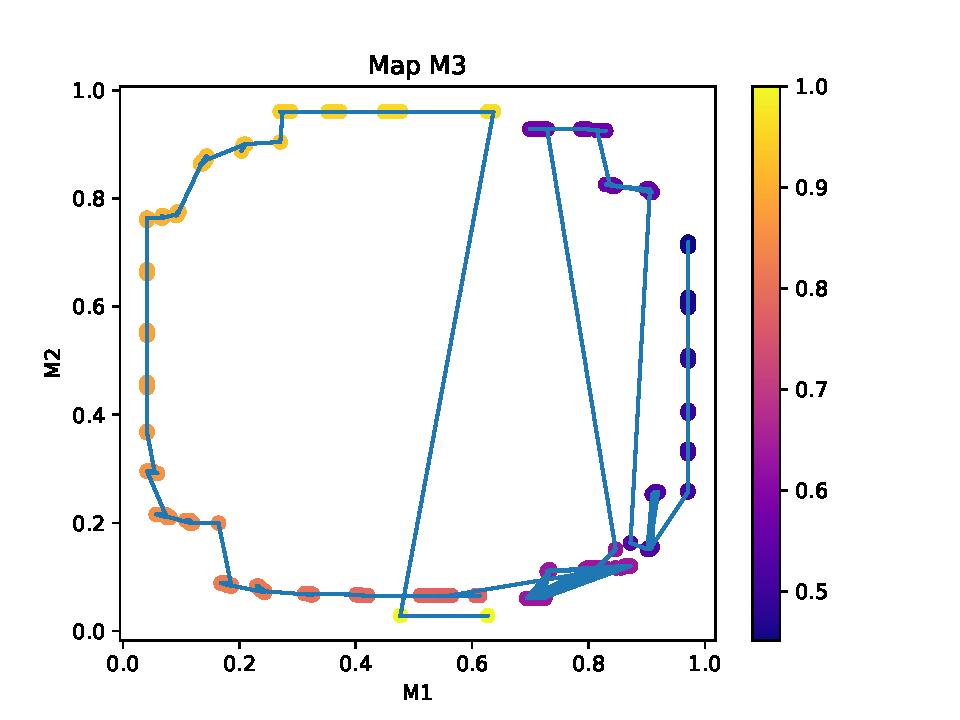
\includegraphics[width=\textwidth]{2som_star_dw3.pdf}
\end{minipage}
\caption{Poids et dépliement des deux cartes lorsqu'elles sont connectées via une carte intermédiaire (architecture (1).}
\end{figure}

% mettre ici figure avec 2 intermédiaires

\begin{figure}[h!]
\begin{minipage}{0.5\textwidth}
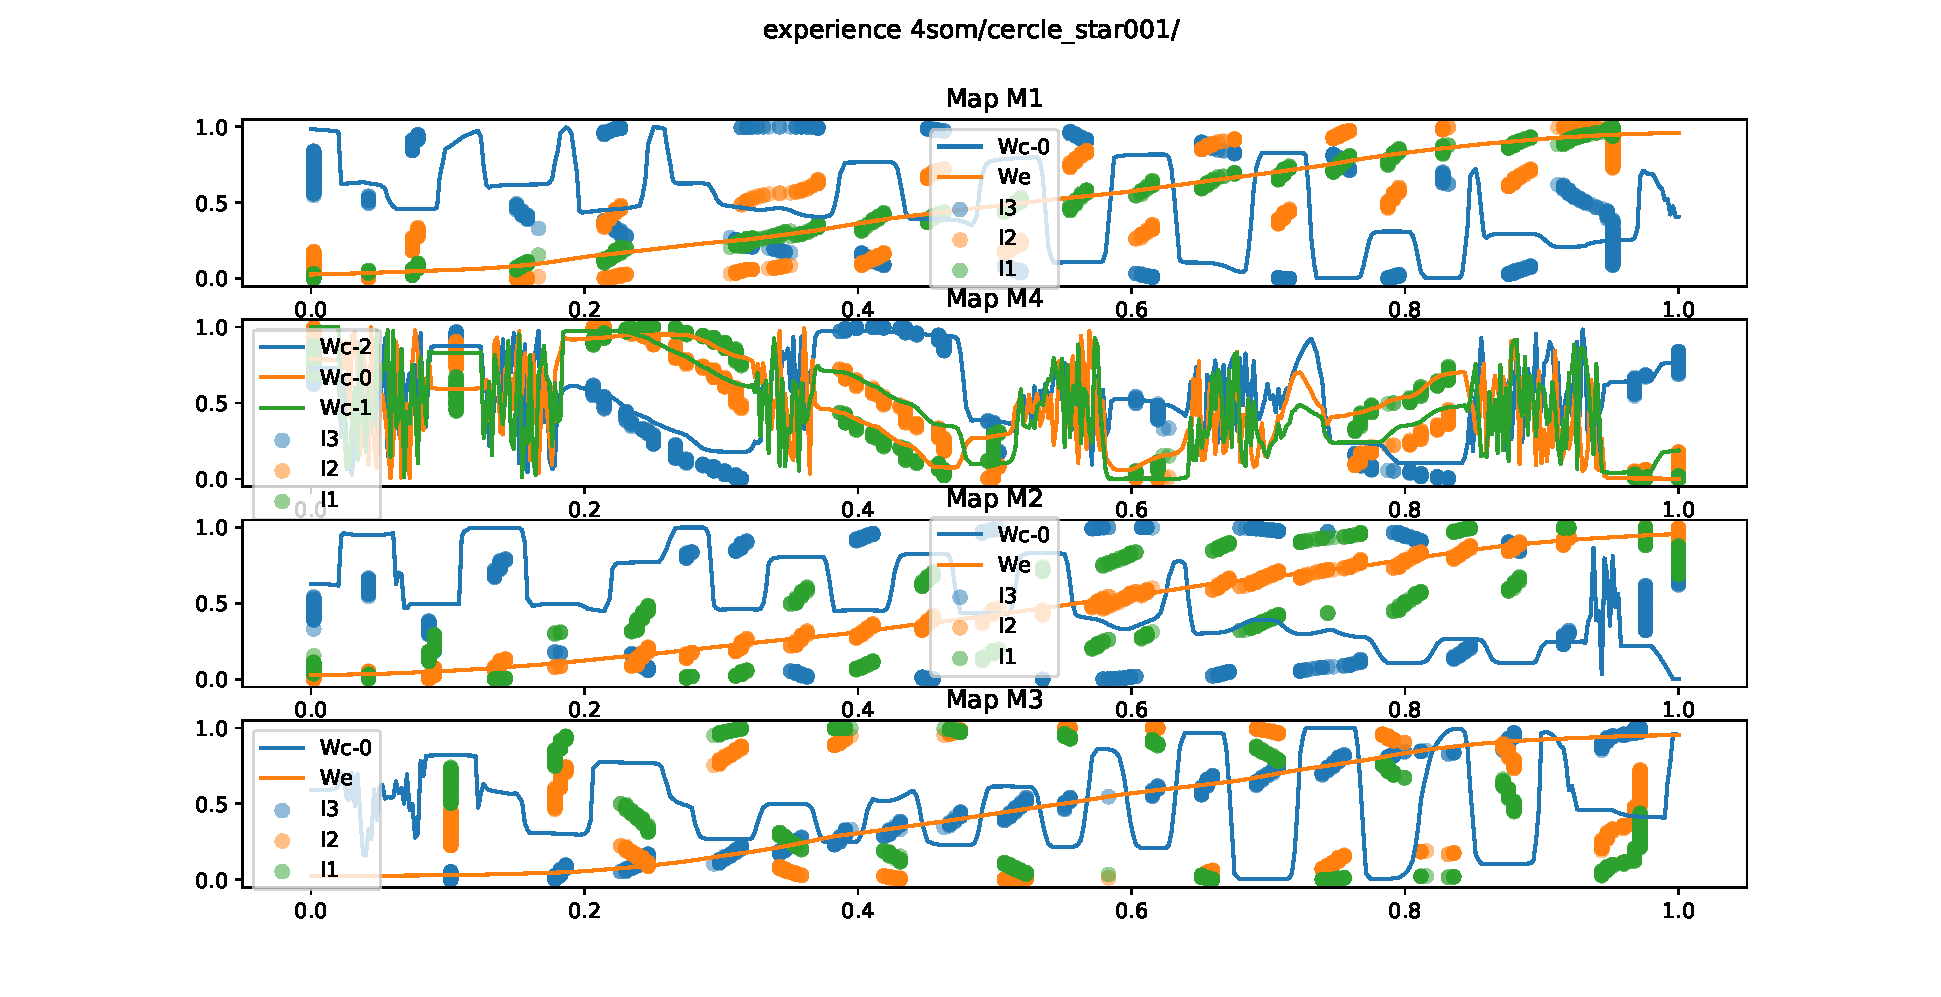
\includegraphics[width=\textwidth]{3som_star_w.pdf}
\end{minipage}
\begin{minipage}{0.5\textwidth}
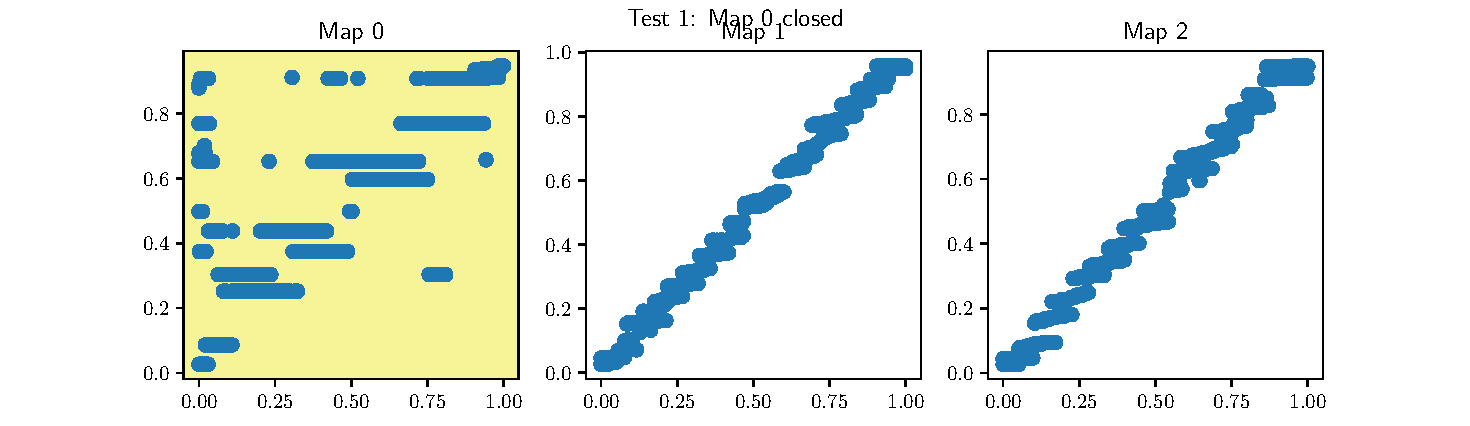
\includegraphics[width=\textwidth]{3som_star_pred.pdf}
\end{minipage}
\caption{Poids et dépliement de trois cartes connectées avec une intermédiaire.}
\label{fig:3som_star}
\end{figure}

\begin{figure}[h!]
\begin{minipage}{0.33\textwidth}
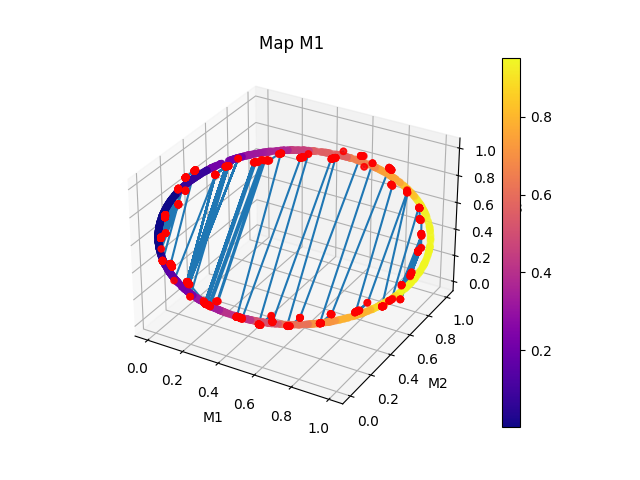
\includegraphics[width=\textwidth]{3som_star_dw1.png}
\end{minipage}
\begin{minipage}{0.33\textwidth}
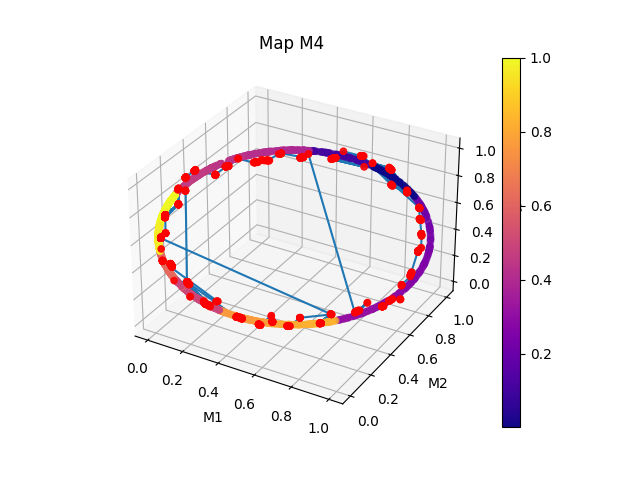
\includegraphics[width=\textwidth]{3som_star_dw4.png}
\end{minipage}
\begin{minipage}{0.33\textwidth}
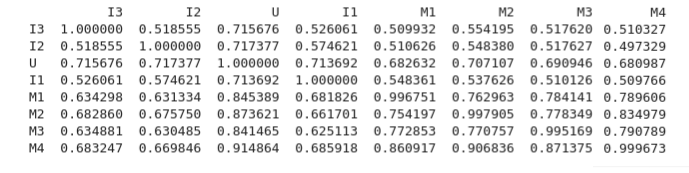
\includegraphics[width=\textwidth]{3som_star_im.png}
\end{minipage}
\label{fig:3som_star_dw}
\caption{Poids et dépliement de trois cartes connectées avec une intermédiaire et information mutuelle. Les cartes 1,2,3 recoivent des entrées, la carte 4 les connecte.}
\label{fig:3som_star}
\end{figure}

Les coefficients d'incertitudes sont ici un élément de comparaison particulièrement bon entre les cartes. Les relations entre les entrées $X$, $Y$ sont identiques, on a en effet la même distribution. 
On peut porter notre attention sur $UC(I1|M1)$ dans les deux cas : ce coefficient est plus élevé dans le cas 2.
Cela traduit une meilleure quantification vectorielle par les cartes ayant une entrée externe lorsqu'on met 2 cartes intermédiaires qu'une seule. On se rapproche en fait d'une architecture dans laquelle les cartes ne seraient pas connectées. Il semblerait donc que seules les connexions directes soient vraiment utiles. 
Par contre, on peut regarder $UC(U|M3)$ pour (1), ou $UC(U|M2)$ et $UC(U|M3)$ pour (2). 
Dans le cas (1) : le coefficient est de 0.93, vs 0.9 sur les deux cartes ayant une entrée externe, donc la différence n'est pas si significative. Les trois cartes ont une information sur le modèle.
Dans le cas (2) : le coefficient est de 0.9 sur M2 et M3, vs 0.8 sur les cartes du bout. Il semble donc que les cartes intermédiaires ont appris une représentation de la variable cachée.

On peut maintenant s'intéresser au dépliement des cartes, et à leur capacité de prédiction dans le cas en 3 dimensions. ( La prédiction n'étant en effet pas possible dans le cas de deux cartes). A trois cartes, la prédiction semble moins bonne que lorsque les trois cartes sont directement connectées. 
Si on regarde les coefficients d'incertitude, on remarque que les BMUs de la carte 4, qui connecte les trois autres, ont une info de 0.9 sur U et sur les bmus des trois autres cartes. Elle possède également un peu plus d'infos sur I1, I2, I3 que les cartes séparées. 
Donc, d'un coté la carte centrale possède les infos sur le modèle, mais d'un autre coté l'architecture effectue mal la prédiction lorsqu'une entrée manque. 

On peut donc imaginer utiliser des cartes centrales dans ce genre d'architecture pour résumer les trois autres. Ainsi, on pourra travailler sur l'info d'une seule des cartes au lieu de trois.

\subsection{Carte contextuelle de rayon 0.2}
Convergence ok, beau sinus de la carte M4 mais plus du tout de prédiction possible. Est ce que ca a un intérêt ? D'un coté, on a résumé les 3 cartes en une seule. 
Cela semble confirmer en tout cas l'implication sous-indices => prédiction. Ici pas de prédiction possible et pas de sous indices. 
 
\subsection{Et si on a la même architecture, avec une carte centrale, mais cette fois les cartes M1, M2, M3 sont également connectées ?}



\subsection{Boucle vs rétroaction à trois cartes}
On a vu avec les cartes intermédiaires que les connexions lointaines semblent jouer un role moins important dans la dynamique que les connexions directe. Ainsi, on peut regarder comment se comporte une architecture de trois cartes connectées en boucle.

\begin{figure}
\begin{minipage}{0.5\textwidth}
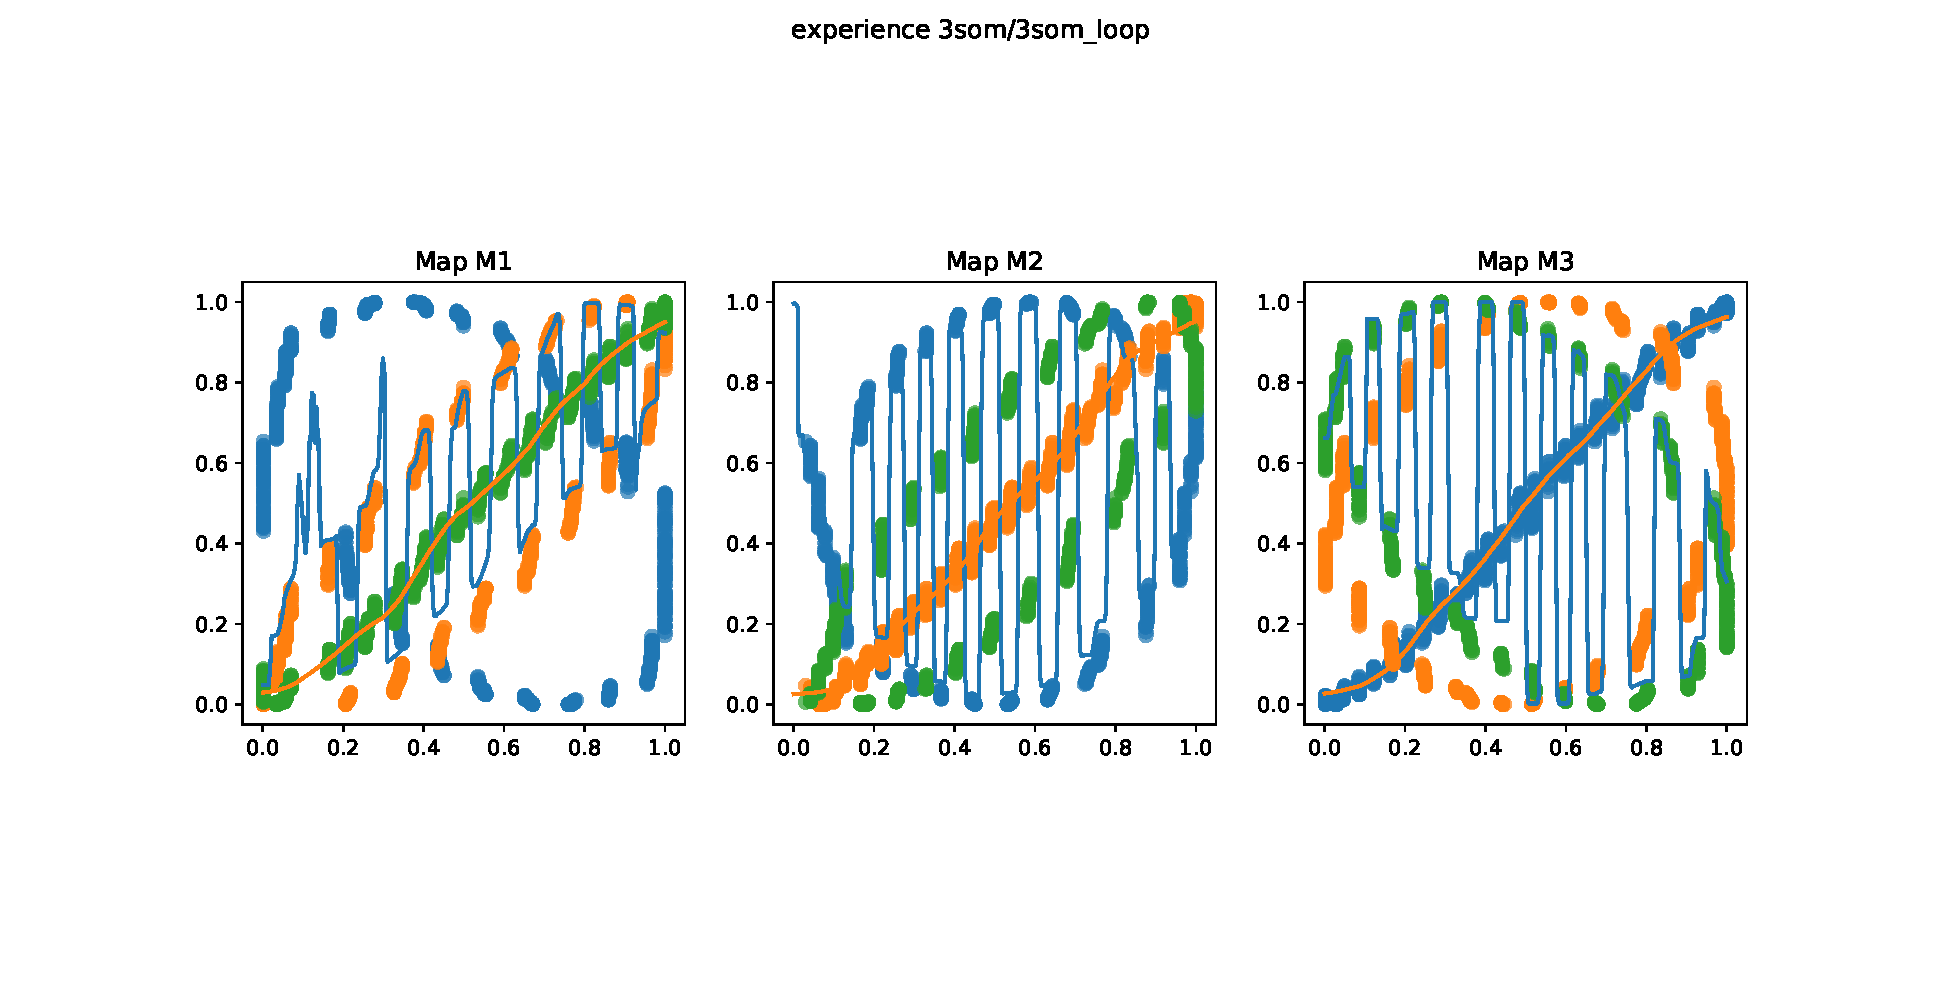
\includegraphics[width=\textwidth]{3som_loop_w.pdf}

\end{minipage}
\begin{minipage}{0.5\textwidth}
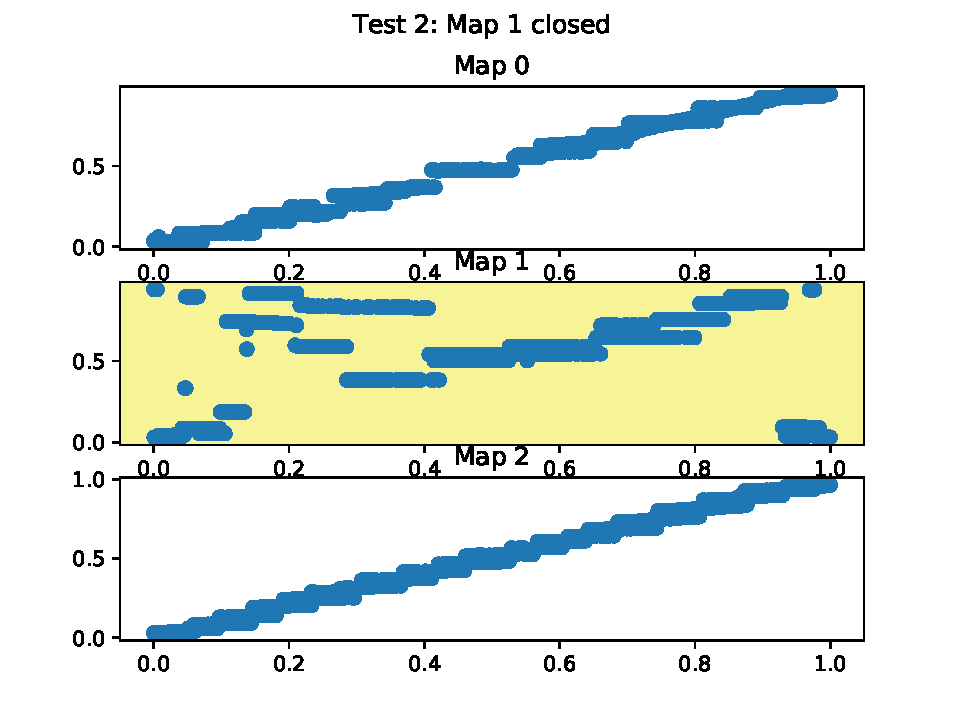
\includegraphics[width=\textwidth]{3som_loop_pred.pdf}
\end{minipage}
\caption{Poids et prédiction de trois cartes connectées en boucle (1-> 2 -> 3 -> 1). L'organisation des poids est semblable à la version en rétroaction, mais la prédiction est plus mauvaise.}
\label{fig:3som_loop}
\end{figure}

\begin{figure}
\begin{minipage}{0.45\textwidth}
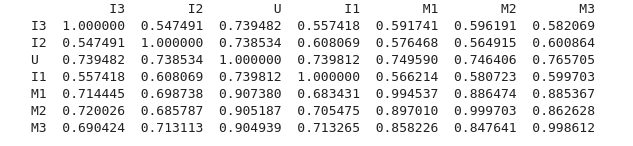
\includegraphics[width=\textwidth]{3som_cercle_im}
\caption{Coefficients d'incertitude lorque les cartes sont connectées rétroactivement, entrées sur un cercle}
\end{minipage}
\hfill
\begin{minipage}{0.45\textwidth}
\centering
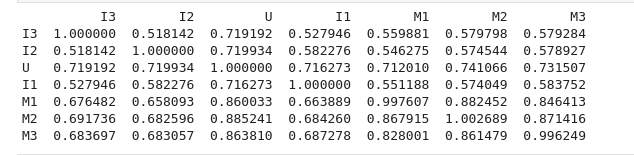
\includegraphics[width=\textwidth]{3som_loop_im.png}
\caption{Coefficient d'incertitude (colonne|ligne) lorsque les cartes sont connectées en boucle, entrées sur un cercle}
\end{minipage}
\end{figure}


\subsection{Conclusion et perspectives: influence de l'architecture}

\section{Influence des paramètres des cartes}

\subsection{rayons de voisinage}
Le rayon de voisinage des cartes, et principalement la différence entre rayons de voisinage externe et contextuel des cartes joue un gros rôle dans l'organisation. C'est cette différence de rayon de voisinage permet la séparation en indices primaires et secondaires. Lorsque les voisinages sont égaux, cette répartition ne se fait pas; mais également, les poids ne peuvent pas se stabiliser. Prendre $r_c < r_e$ permet donc une organisation stable, une séparation d'indices et une prédiction. Les paramètres sont indiqués en tableau~\ref{tab:rcre_params}.

\emph{vidéo rcre}
\begin{table}
\begin{tabular}{ l c c c }
 name & re & rc & delta\\ 
 rcre0 & 0.2 & 0.1 & 0.1\\  
 rcre1 & 0.2 & 0.07 & 0.1 \\
 rcre2 & 0.2 & 0.05 & 0.1 \\
 rcre3 & 0.2 & 0.01 & 0.1 \\
 rcre4 & 0.2 & 0.005 & 0.1
\end{tabular}
\caption{Paramètres de rayon de voisinage utilisés dans les expériences de comparaison}
\label{tab:rcre_params}
\end{table}

\subsection{Taille de la carte}

Carte grande taille, même comportement qu'avec 500 noeuds; pas d'améloriation significative.
Carte petite taille (20 noeuds) :on n'a pas assez d'unités pour faire les séparations. On a donc 8 unités qui seront bmus, mais pas de prédiction possible ou de différenciation de U par exemple. (voir figures).
Ainsi, le comportement auquel on s"intéresse, à savoir la capacité de différentiation des BMU selon le modèle, n'est plus possible. Cela pose question  :
\begin{itemize}
\item Si on veut faire des cartes 2D, on devra donc avoir des grandes cartes (100 par 100 au moins)! 
\item Même sur 500 points, on a seulement ~20 régions d'une carte qui sont utilisées, et parmi elle peu de BMU. On perd beaucoup de noeuds.
\item Si les entrées sont trop complexes (beaucoup de cartes, donc beaucoup de valeurs possible pour U), pourra t on toujours effectuer une différencitation des entrées ? 
\end{itemize}



\subsection{Combinaison des activités externes et contextuelles par moyenne ou moyenne géométrique}

\subsection{Influence de la relaxtion}

Il semble que la relaxation ne soit même plus utile lorsque 

\section{Conclusion des expériences, perspectives et limites}
\chapter*{Conclusion}

\section*{Résumé des contributions et discussion}

La thèse que nous avons présentée se penche sur la problématique de développement d'un mécanisme d'apprentissage au sein d'une architecture de cartes non-hiérarchiques.
Nous avons choisi de construire un modèle d'architectures prenant la position du BMU comme contexte transmis entre les cartes et avons construit un modèle s'appuyant sur une recherche de consensus entre cartes. 
Ce choix de modèle repose sur les travaux conduits précédemment dans l'équipe, des architectures de SOM cellulaires calculant leurs activations grâce à des DNF couplés. 
Le couplage de ces DNF induisait un mécanisme de relaxation au sein de cartes pour trouver un BMU satisfaisant toutes les cartes. L'architecture de SOM proposée remplace les DNF par un calcul d'argmax mais conserve l'aspect relaxation pour lier les cartes entre elle en architecture. La position du BMU apparaît par ailleurs comme un contexte transmis dans de nombreux modèles d'architecture de cartes hiérarchiques et récurrentes. Enfin, la position du BMU est une valeur exploitant totalement l'aspect organisé de la carte de Kohonen et est une valeur légère à transmettre entre les cartes, car il s'agit d'un réel ou d'une valeur 2D.

Nos travaux sont ainsi partis d'un modèle, construit à partir de la littérature et des études précédentes~; les travaux présentés dans cette thèse cherchent à étudier le comportement du modèle en vue d'applications ou de développement futurs.
Nous nous sommes concentrés sur une tâche particulière nous semblant intéressante à réaliser à base d'architectures multi-cartes~: l'apprentissage de représentations multimodales.

Les travaux présentés dans ce manuscrit détaillent le comportement de l'architecture sur des structures comportant un faible nombre de cartes.
Les contributions de ces travaux sont les suivantes~: 
Nous avons détaillé le modèle et analysé comment la relaxation permet de trouver un BMU dans chaque carte. Nous avons souligné l'importance de garder l'activation externe des cartes prépondérante face à l'activité contextuelle, qui vient seulement moduler l'activité externe

Nous avons ensuite défini un cadre d'application multimodal de l'architecture de cartes, l'apprentissage multimodal. Nous proposons de nous intéresser à des entrées ayant une dépendance et représentons cette dépendance comme une paramétrisation de dimension inférieure du modèle.
Le chapitre \ref{chap:repr} présente la méthode d'analyse du comportement des cartes sur des applications multimodales jouets et des représentations. Nous avons vu que contrairement à l'analyse classique des cartes de Kohonen qui s'appuie sur l'organisation des poids des cartes, nous avons préféré nous intéresser au comportement de l'architecture de cartes lors de phases de tests. Cette méthode modélise les entrées et les éléments des cartes comme des variables aléatoires dont nous avons ensuite cherché à tracer les dépendances.
Nous avons ensuite détaillé le comportement d'architectures de deux et trois cartes sur des données jouet pour en extraire les comportements d'apprentissage principaux et l'influence de certains paramètres d'apprentissage.
Les comportements observé lors de cet étude sont les suivants~: 
\begin{itemize}
    \item Pour faire émerger un apprentissage du modèle d'entrée et non seulement de l'entrée externe, nous voulons prendre un grand rayon de voisinage externe $r_e$ face au rayon contextuel $r_c$. Cette différence d'échelle entre paramètres induit une organisation subordonnée des poids contextuels face aux poids externes lors de l'apprentissage, conduisant les cartes à s'organiser selon deux échelles d'indices. Une carte s'organise ainsi globalement selon la valeur de ses entrées externe mais sépare également la position des BMUs selon la valeur générale du modèle d'entrée.
    \item Cette séparation des BMUs intervient dès qu'une carte doit différencier une même valeur de son entrée externe, correspondant à plusieurs points différents du modèle d'entrée. Dans ce cas, la carte forme plusieurs sous-cartes mappant un ensemble de valeurs de l'entrée externe à toutes les valeurs de $U$ correspondant à cet intervalle. Cette organisation en zones est un compromis entre encodage de $U$ et qualité de la quantification vectorielle sur $\inpx$, dont la qualité est réduite par rapport à une carte classique. Dans le cas ou le modèle d'entrée ne nécessite pas cette séparation, une carte se comporte comme une carte classique.
    \item Grâce à ces deux échelles de quantification vectorielle, une architecture CxSOM est capable de générer une prédiction dans une des cartes de l'architecture à laquelle on n'a pas présenté d'entrée externe lors du test.
    Cette prédiction est cohérente avec le modèle d'entrée, et n'est possible que grâce à l'organisation des cartes en "zones". Grâce aux rétroactions, une carte acquiert ainsi une capacité de prise de décision sans avoir besoin d'un algorithme supplémentaire analysant la sortie des cartes. Cette capacité n'est pas permise par des architectures feed-forward ou des cartes classiques. 
    \item Nous avons mis en évidence que le comportement généré par les cartes en une dimension s'étend aux cartes en deux dimensions, généralement utilisées en pratique. Ce comportement est prometteur pour la mise en pratique des architectures de cartes sur des données de plus grande dimension.
\end{itemize}

Nous avons ensuite mis en pratique la capacité de prédiction sur un exemple d'application. Lors du déplacement d'un drone sur une trajectoire définie, la valeur de la commande à envoyer dépend des valeurs des capteurs, formant des entrées multimodales. Nous avons utilisé une architecture de quatre cartes pour apprendre les relations entre commande et entrées et utilisé la prédiction pour prédire la commande à envoyer au drone. Cette expérience nous a permis de tester une mise en situation réelle de l'architecture de carte et a montré une capacité de réaction en temps réel correcte. Du travail autour de la stabilisation des commandes, de choix de capteurs à considérer, serait nécessaire pour une véritable application robotique, mais cette expérience constitue un premier exemple de mise en situation réelle de l'architecture CxSOM.

Nous avons enfin étudié plusieurs méthodes numériques cherchant à évaluer l'encodage du modèle d'entrée au sein de l'architecture de cartes, dans l'optique de disposer d'un indicateur permettant de comparer des expériences entre elles, se passer de représentations graphiques, limitées aux valeurs 1D et 2D, pour caractériser l'apprentissage sur des données de grande dimension, et par exemple permettre l'optimisation automatique des paramètres. Ces indicateurs s'appuient sur la modélisation statistique des entrées et sorties des cartes.
Comme nous avons observé que l'apprentissage dans une architecture de deux cartes est marquée par une relation fonctionnelle entre $U$ et le BMU $\bmu$ dans chaque carte et avons ainsi utilisé le ratio de corrélation, qui permet de quantifier à quel point $U$ est une fonction du BMU dans chacune des cartes.
Cette valeur mesure bien cette relation fonctionnelle mais doit être utilisée en comparaison avec le ratio de corrélation entre $U$ et $\inpx$ afin de vérifier la relation fonctionnelle d'origine entre le modèle et l'entrée présentée à la carte.
Nous avons également étudié un indicateur s'appuyant sur l'information mutuelle normalisée dans chaque carte. Cependant, l'observation que $U$ est une fonction du BMU dans chaque carte n'est pas forcément générale à des architectures comportant plus de cartes, et surtout n'est pas souhaitable.
Nous avons mesuré l'information mutuelle entre $U$ et $\bmu$ dans chaque carte de l'architecture.

Ce modèle de représentation est intéressant pour :
\begin{itemize}
    \item 
\end{itemize}

Par contre, il montre certaines limites, déjà sur plusieurs cartes : 
\begin{itemize}
    \item Beaucoup de n\oe{}uds morts. La carte prend ici le rôle d'un mapping. On pourrait imaginer des modèles d'apprentissage simulant le coté + continu, par exemple avec des poids dans les arêtes des cartes qui permettraient d'utiliser tous les n\oe{}uds.
    \item Rigidité qui limite l'apprentissage de $U$ en grande dimension.
\end{itemize}


% conclusion générale.

\section*{Perspectives}

Les perspectives à court terme de ces travaux sont de continuer le développement du modèle en s'intéressant aux connexions au sein d'une architecture comportant de plus nombreuses cartes.
Le nombre de connexions possible au sein d'une architecture comportant un nombre fixé de cartes est exponentiel et chaque configuration peut complètement modifier la façon dont se comporte l'architecture. Par ailleurs, certaines cartes peuvent ou non prendre des entrées externes, ajoutant un grand nombre de configurations possibles à explorer. Grâce à nos travaux, nous avons une idée des paramètres à utiliser dans l'architecture et des sorties pertinentes à considérer pour étudier le comportement d'apprentissage. Nous disposons aussi d'une librairie performante pour construire les architectures de cartes, développée en parallèle de la thèse au sein de l'équipe de recherche.
L'étude de plus grandes architectures devra se faire d'un point de vue plus global, en s'appuyant sur le comportement général de l'architecture et non seulement d'un point de vue d'une carte. Il reste à définir les cas d'études sur lesquels appliquer ces architectures à grande échelle.
L'aspect modulaire de ces architectures pourrait par exemple nous faire envisager des modules d'interaction avec l'environnement, qui traitent les entrées sensorielles et des modules d'apprentissage, en s'inspirant des structures fonctionnelles observées en biologie.
Pour cela, nous avons vu qu'il sera pertinent de s'intéresser à l'information au sein du système de cartes à partir du modèle d'entrée et des positions de BMU représentant l'état des cartes du système.

Un des objectifs à long terme du développement d'architectures multi-cartes est également l'intégration de connexions récurrentes entre cartes, afin de traiter des données séquentielles. L'utilisation de la position du BMU comme interface a en effet été utilisée au sein de modèles de cartes récurrentes telles que SOMSD~; ce modèle ainsi que son adaptation sur deux cartes ont fait l'objet d'études précédentes dans notre équipe \cite{baheux_towards_2014, fix20}. 
Dans ces modèles de cartes récurrentes, la carte prend en entrée externe un élément d'une séquence d'entrée et comme entrée contextuelle la position du BMU obtenu lors de l'itération précédente.
Les propriétés d'organisation observées sur ce type de cartes récurrentes rejoignent celles observée dans l'architecture CxSOM~: une carte distingue son BMU en fonction de l'entrée externe mais également en fonction de sa place dans la séquence d'entrée.
Une perspective d'étude sera ainsi d'associer des connexions temporelles et des connexions multimodales au sein d'une architecture de cartes afin de traiter des données séquentielles.
Un inconvénient des cartes récurrentes simple est leur oubli de la séquence une fois que cette dernière n'a pas été présentée. 
Une architecture de cartes pourrait par exemple apporter des modules de mémoire supplémentaire pour l'apprentissage d'un ensemble de séquences \cite{Ellefsen2015NeuralMH}.
Une direction d'application d'architectures de cartes peut être la construction d'un système d'apprentissage \og sur le long terme \fg{} , apprenant au cours du temps des entrées et sorties et pouvant générer des prises de décision dans le système.

Enfin, l'architecture que nous avons proposée s'appuie uniquement sur des cartes auto-organisatrices. Nous pouvons envisager de coupler les mécanismes induits par l'architecture de cartes à d'autres mécanismes d'apprentissage. L'inspiration biologique 

% Résumé des contributions et synthèse : 


% Perspectives des travaux : 

% Mémoire associative pas forcément le cas d'étude le plus adapté à un contexte de modularité.
% Mémoires temporelles, interactions avec environnement vs modules d'apprentissage, \cite{Ellefsen2015NeuralMH}
% Apprentissage sur le long terme.

% Proximité avec modules récurrents pour une généralisation du modèle.
% Perspective : envisager d'autres cas d'utilisation du modèle, qui induisent d'autres architectures.
\bibliography{biblio_modularite.bib}
\bibliographystyle{plain}
\end{document}